\appendix
\numberwithin{equation}{section}

\section{Xenon recoil and matching checks}
\label{sec:matching}

\begin{figure}[tbp]
\centering
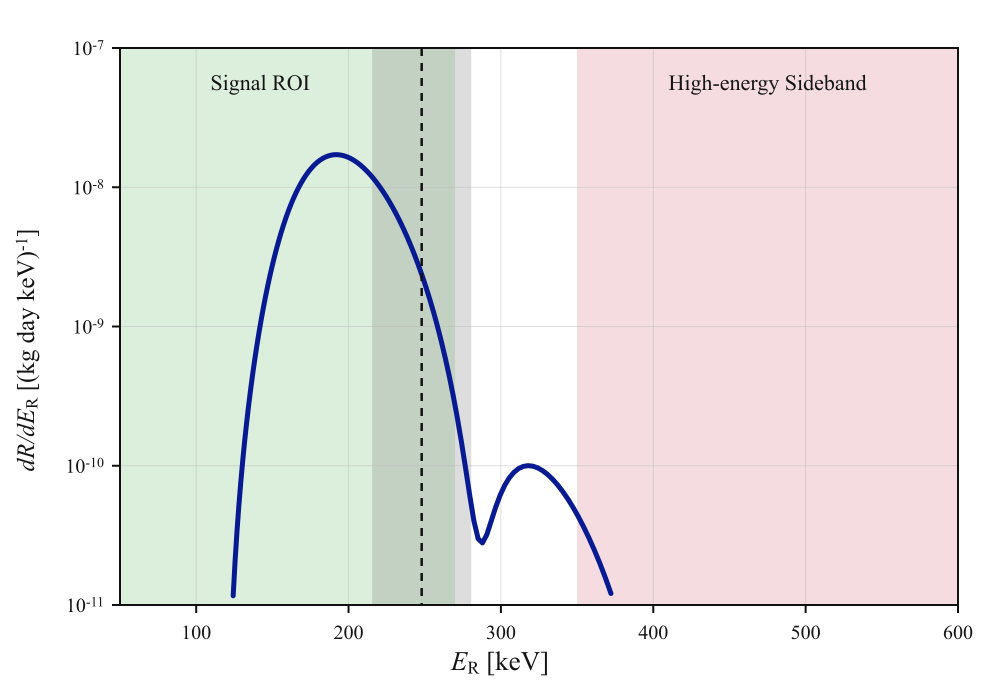
\includegraphics[width=.58\linewidth]{figures/a01_original_recoil.png}
\caption{Independent reproduction of the universal-vector reference benchmark, used to check the recoil shape and units.}
\label{fig:reference_recoil}
\end{figure}

After subtraction at zero momentum, the finite heavy-quark contribution to photon mixing is

\begin{equation}
\label{eq:finite_mixing}
\begin{aligned}
\delta d_{cbt}(s)&=-\frac{2\alpha}{\pi}\sum_{q=c,b,t}N_cQ_q\frac{\widehat m_q}{m_t}\\
&\quad\times\int_0^1 dx\,x(1-x)\log\left[1-\frac{s x(1-x)}{\widehat m_q^2}-i0\right].
\end{aligned}
\end{equation}

\begin{figure}[tbp]
\centering
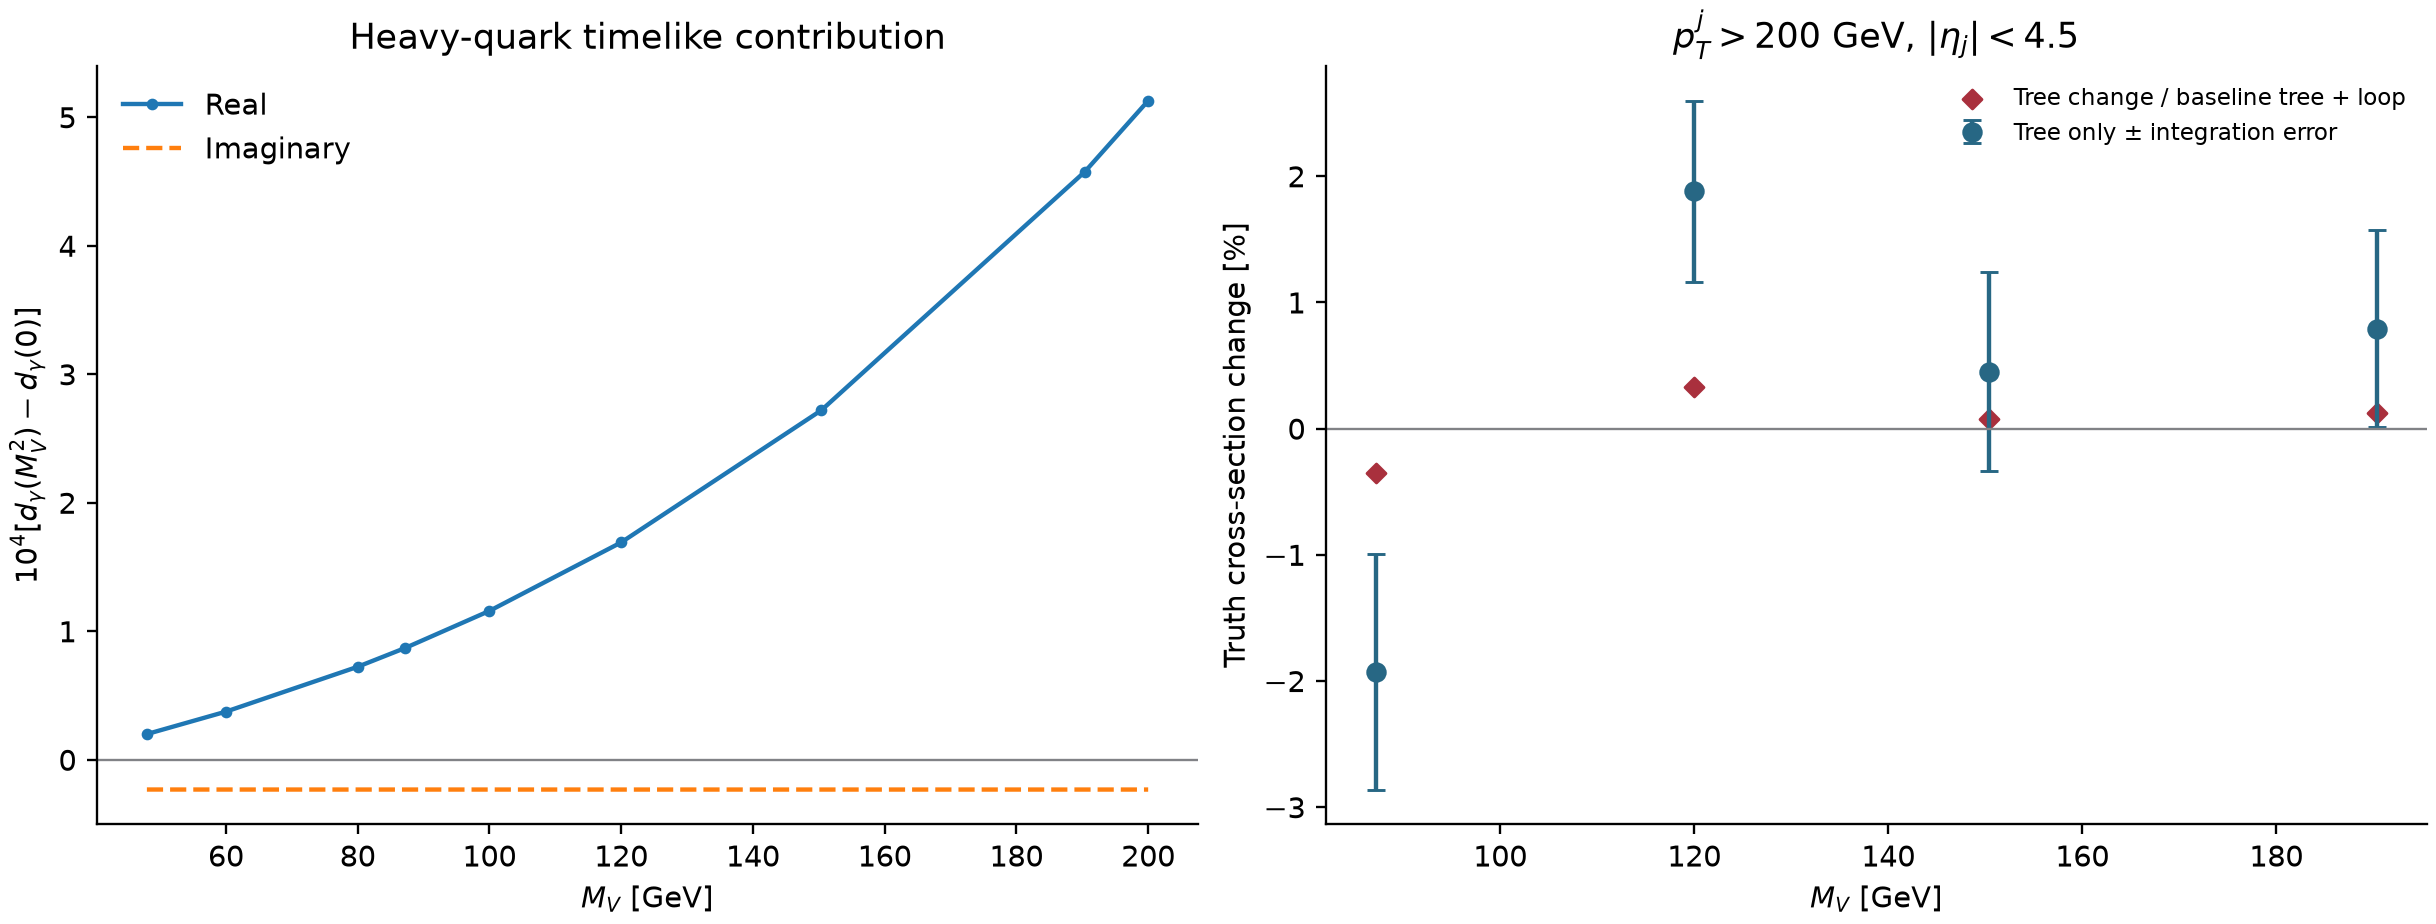
\includegraphics[width=.86\linewidth]{figures/a02_timelike_mixing.png}
\caption{At four on-shell masses we include $\delta d_{cbt}(M_V^2)$ in the $pp\to Vj$ tree amplitude. For $p_T^j>200$ GeV, the tree cross section changes by about $2\%$ or less. Relative to the original tree-plus-loop cross section, the shift is below $0.4\%$. For the relic calculation, we approximate the finite term by its real part evaluated at the dark-pair threshold or at the mediator pole. The largest shifts in $\Omega h^2$ across the four points are $1.12\times10^{-4}$ and $4.64\times10^{-4}$, respectively. Lowering \texttt{Beps} by two orders of magnitude changes the abundance by less than $2\times10^{-11}$ at three numerical benchmarks.}
\label{fig:timelike}
\end{figure}

\begin{figure}[tbp]
\centering
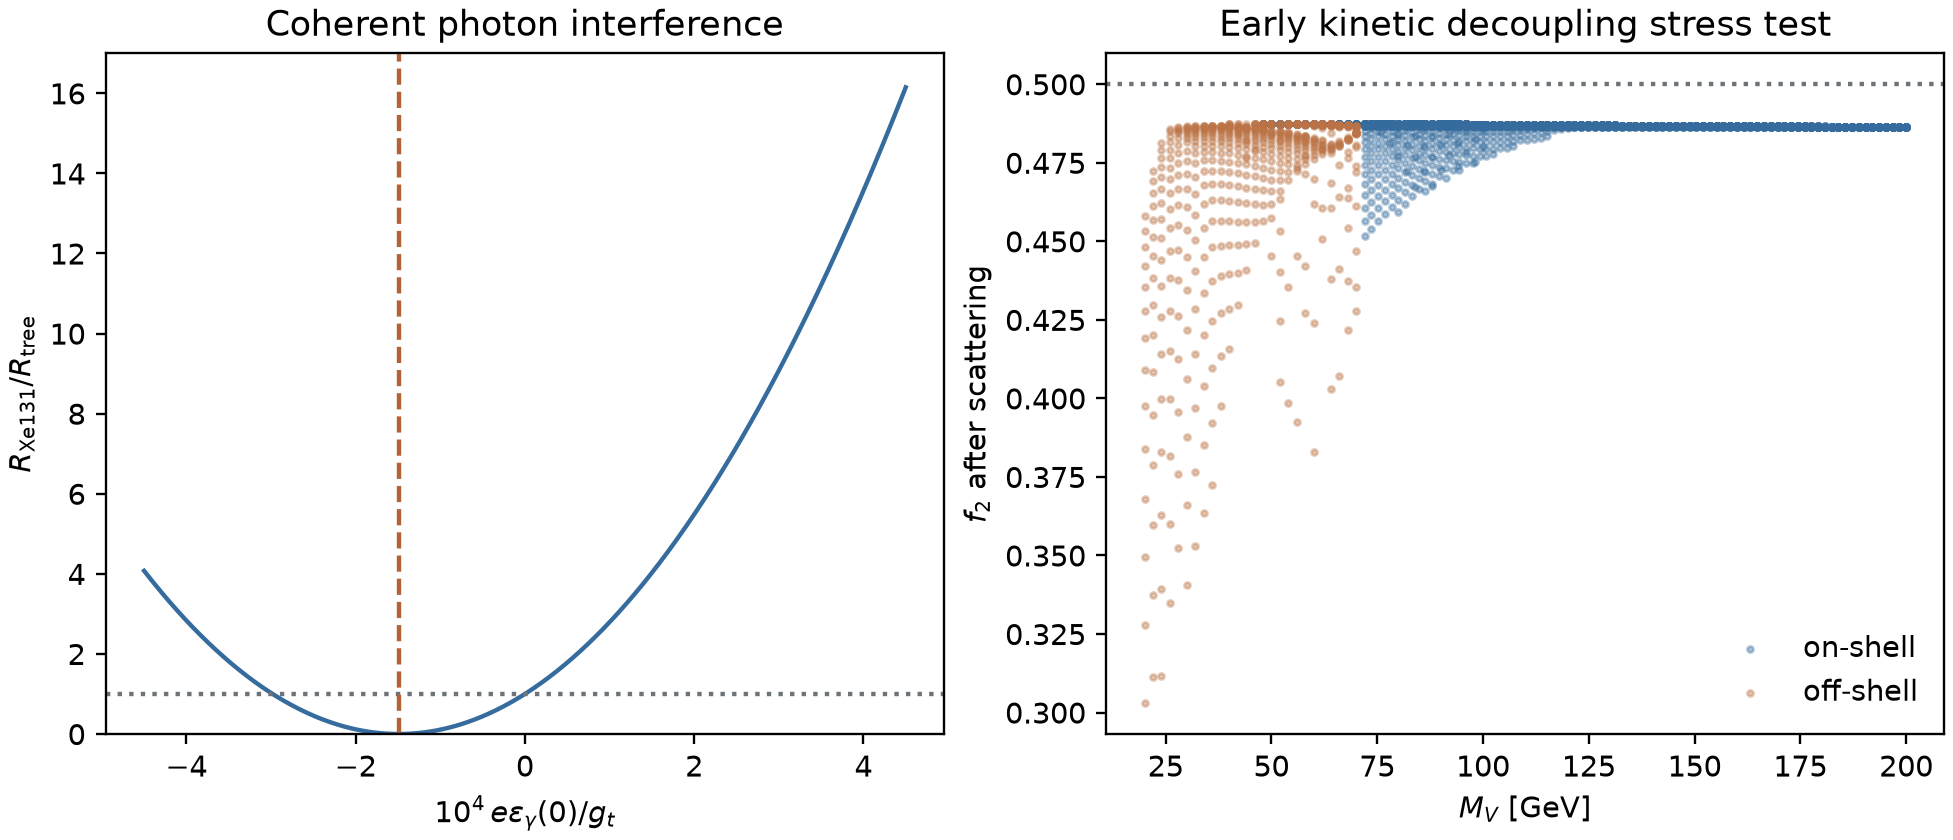
\includegraphics[width=.86\linewidth]{figures/a03_excited_fraction.png}
\caption{The conversion $\chi_2\chi_2\leftrightarrow\chi_1\chi_1$ can change the excited-state fraction after chemical freeze-out. In the standard thermal histories tested, with additional decay suppressed and the Standard Model bath included, the minimum at the on-shell benchmarks is $f_2\simeq0.45$ and falls to about $0.30$ at some off-shell benchmarks. The splitting $\Delta m<2m_e$ closes the electron-pair decay channel. Independent $V$--$Z$ mixing or a transition dipole can still affect the lifetime. \cite{gemmell2026,carrillo2022}}
\label{fig:fraction}
\end{figure}

After the total abundance freezes out, detailed balance for dark-state conversion gives $\dot f_2=-n_\chi\langle\sigma v\rangle_{22\to11}[f_2^2-e^{-2\Delta m/T_\chi}(1-f_2)^2]$, where $T_\chi$ is the dark-sector kinetic temperature. We model conversion with Born contact scattering and vary the assumptions about kinetic decoupling. The resulting $f_2$ values serve as benchmarks for those thermal histories.

\begin{figure}[tbp]
\centering
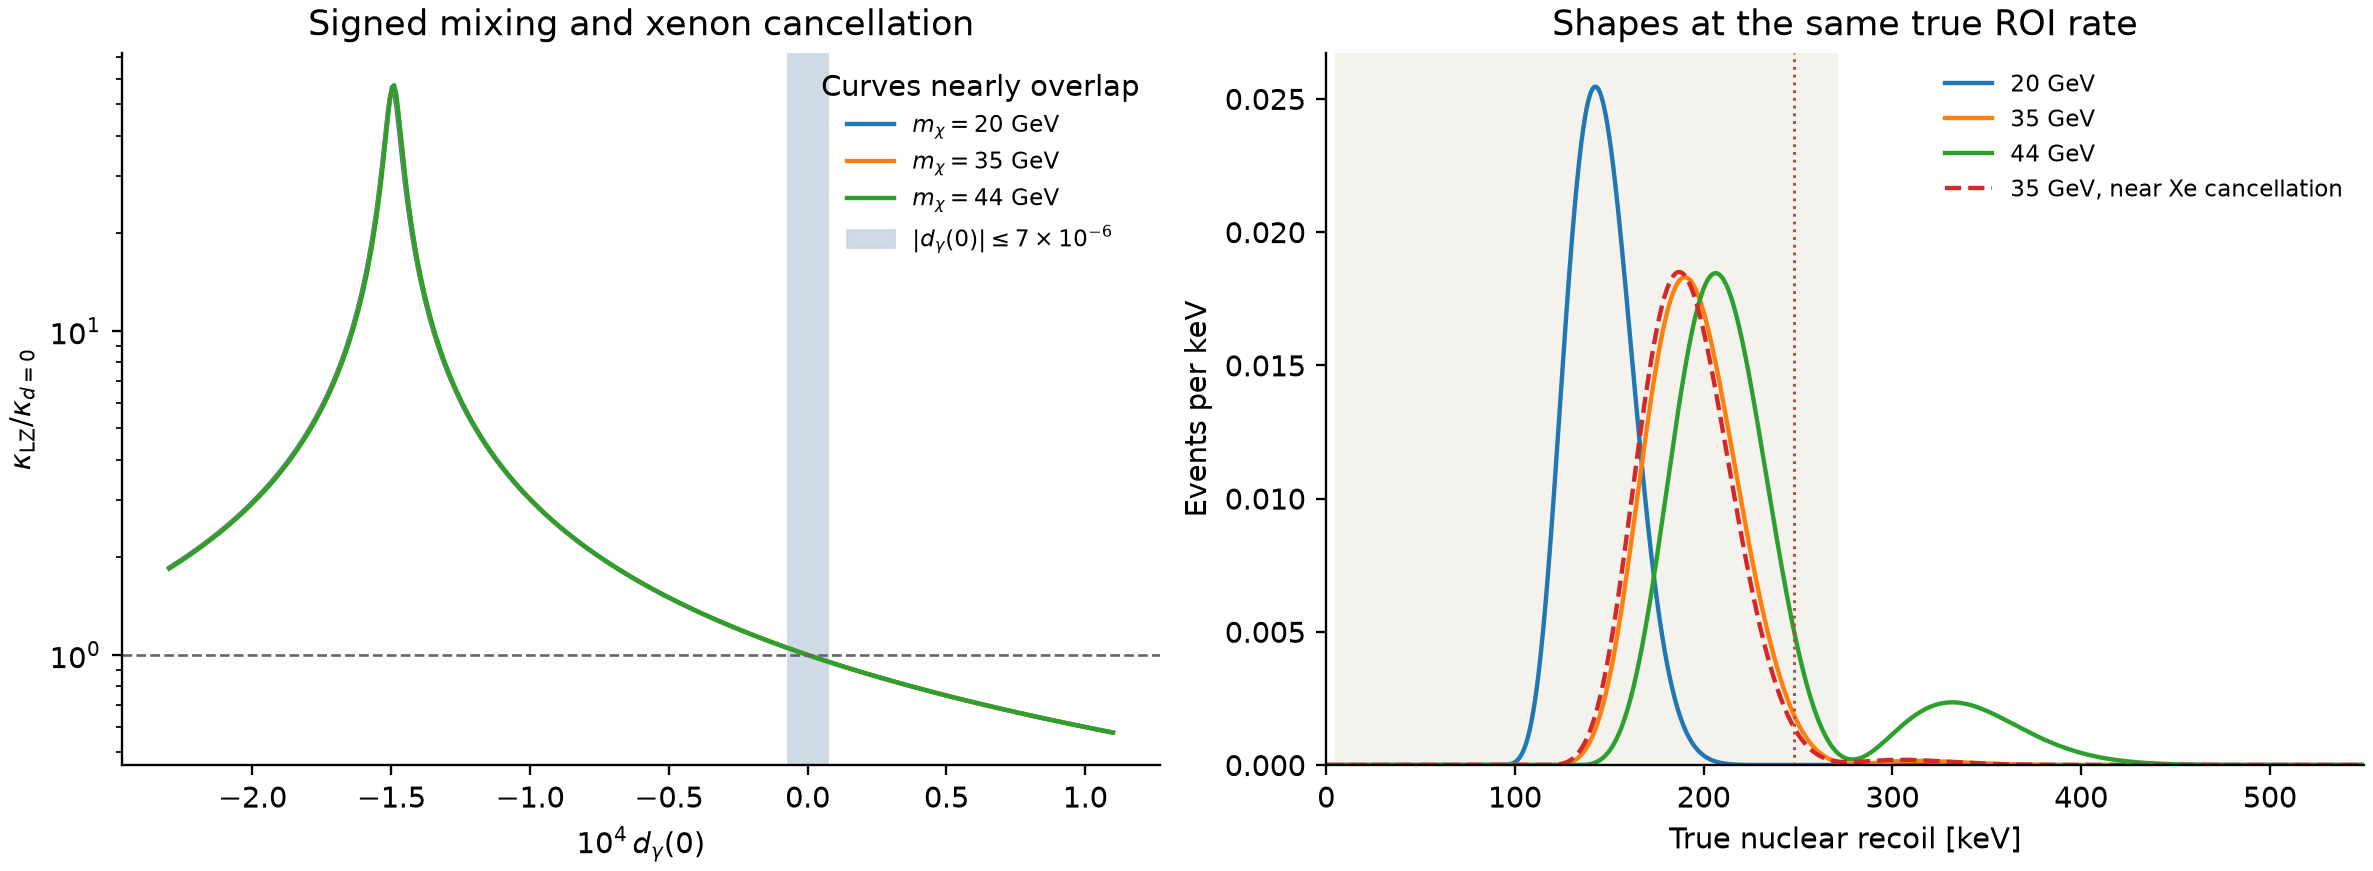
\includegraphics[width=.86\linewidth]{figures/06_matching_and_spectra.png}
\caption{The left panel shows how photon mixing changes the coupling required to match the yield. The right panel compares spectra with the same integrated truth-level yield. After Gaussian smoothing with a width of 32.5 keV, the signal densities near 248 keV at $m_\chi=20,35,44$ GeV are approximately $2.75\times10^{-4}$, $4.54\times10^{-3}$, and $6.98\times10^{-3}$ events/keV. The energy-spectrum approximation uses Gaussian smoothing alone. The LZ S1/S2 response and backgrounds enter an event-level analysis.}
\label{fig:mixing}
\end{figure}

\begin{figure}[tbp]
\centering
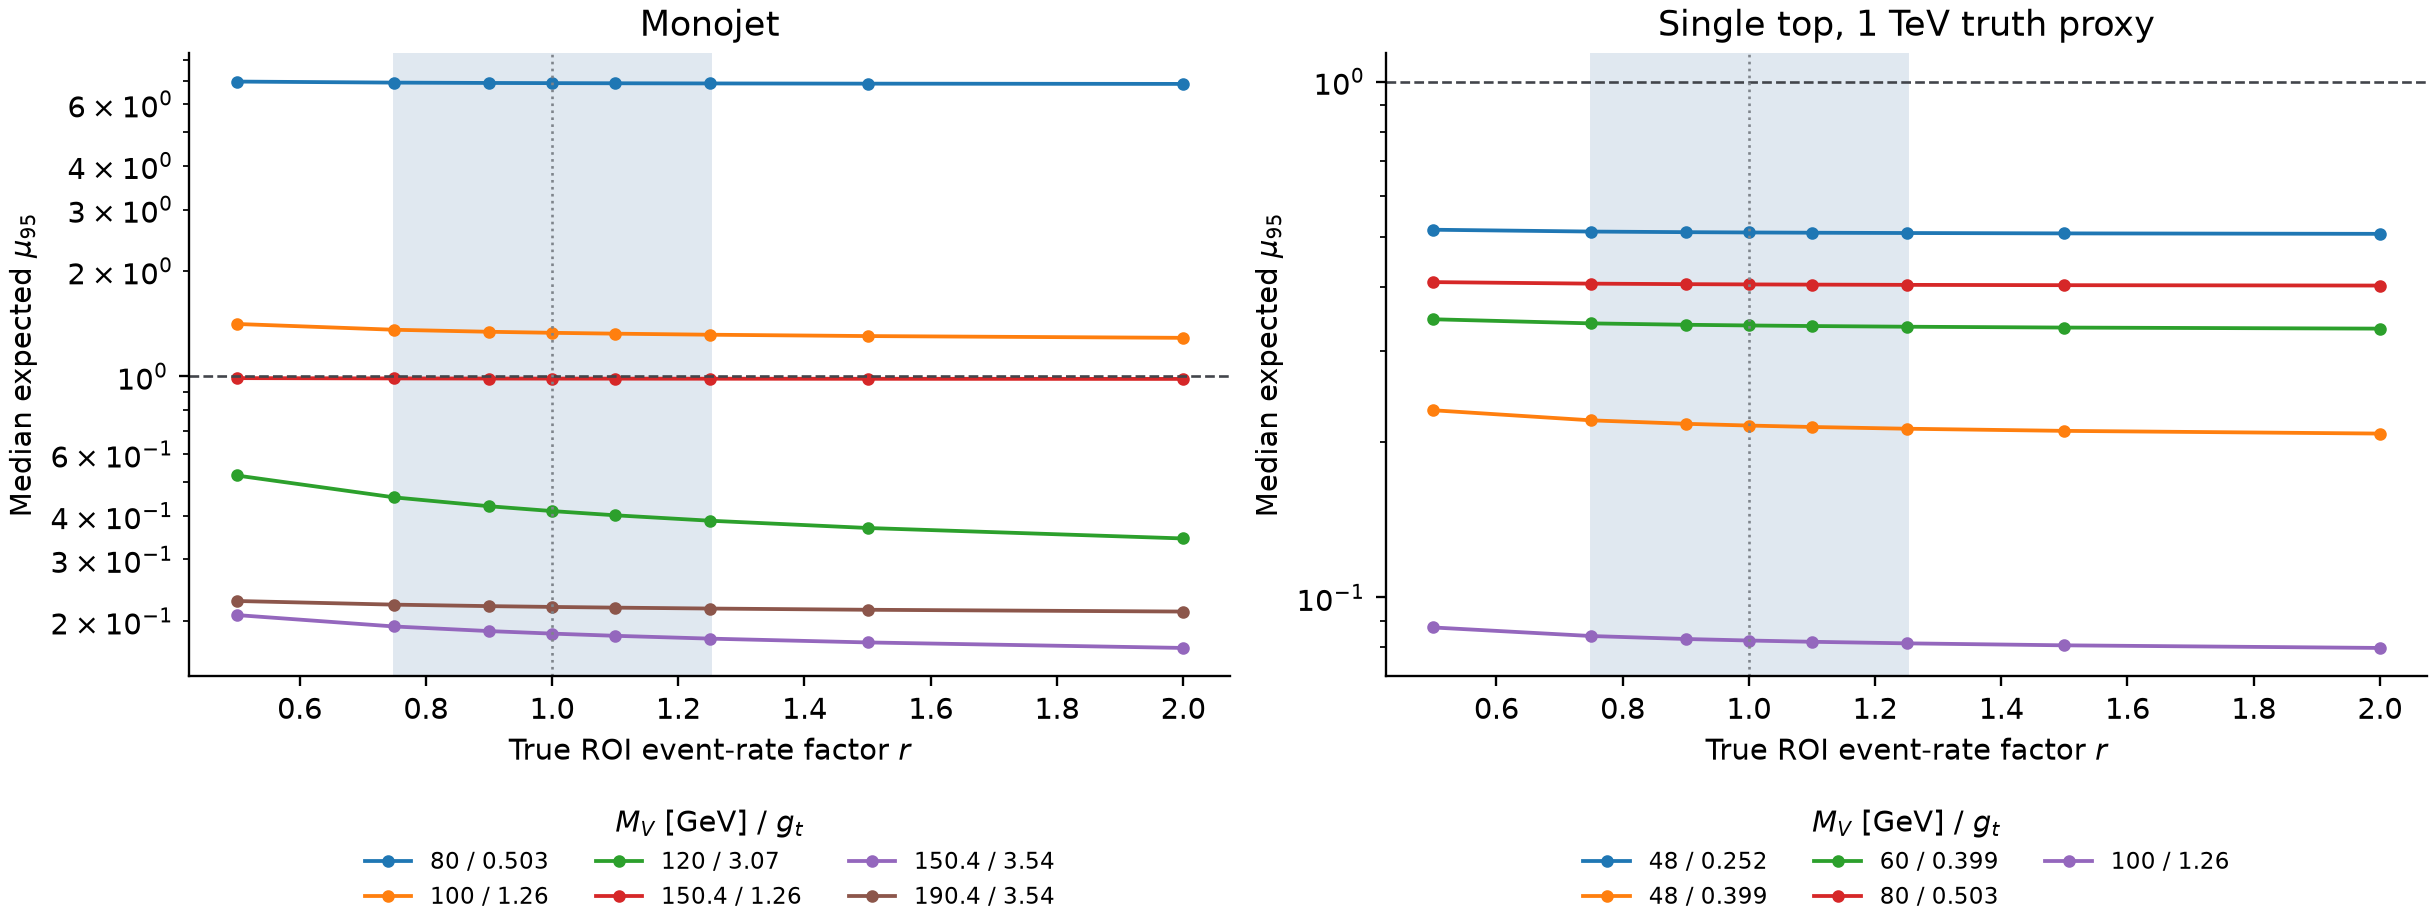
\includegraphics[width=.86\linewidth]{figures/07_lz_rate_variation.png}
\caption{We solve for the central Planck abundance and compute the CMS limit for each on-shell point at each fixed target yield. The shaded interval $r=0.75$--$1.25$ is the prescribed range for the normalization test, corresponding to $0.84$--$1.40$ expected truth-level events.}
\label{fig:rate}
\end{figure}

\section{Cross-section cuts and the mass projection}
\label{sec:production_checks}

The UFO for the closed quark loop includes a rational $R_2$ vertex for $gggV$ for each quark flavor. We replace the photon vector coupling in \texttt{loop\_sm} to obtain the coefficient $i g_{Vq}g_s^3/(48\pi^2)$ per flavor, with color structure $d^{abc}$. Including this term gives a numerical Ward/BRS test ratio of about $6.3\times10^{-24}$ for $gg\to gV$ at $M_V=87.18$ GeV and a partonic energy of 1 TeV. \cite{hirschi2015}

\begin{figure}[tbp]
\centering
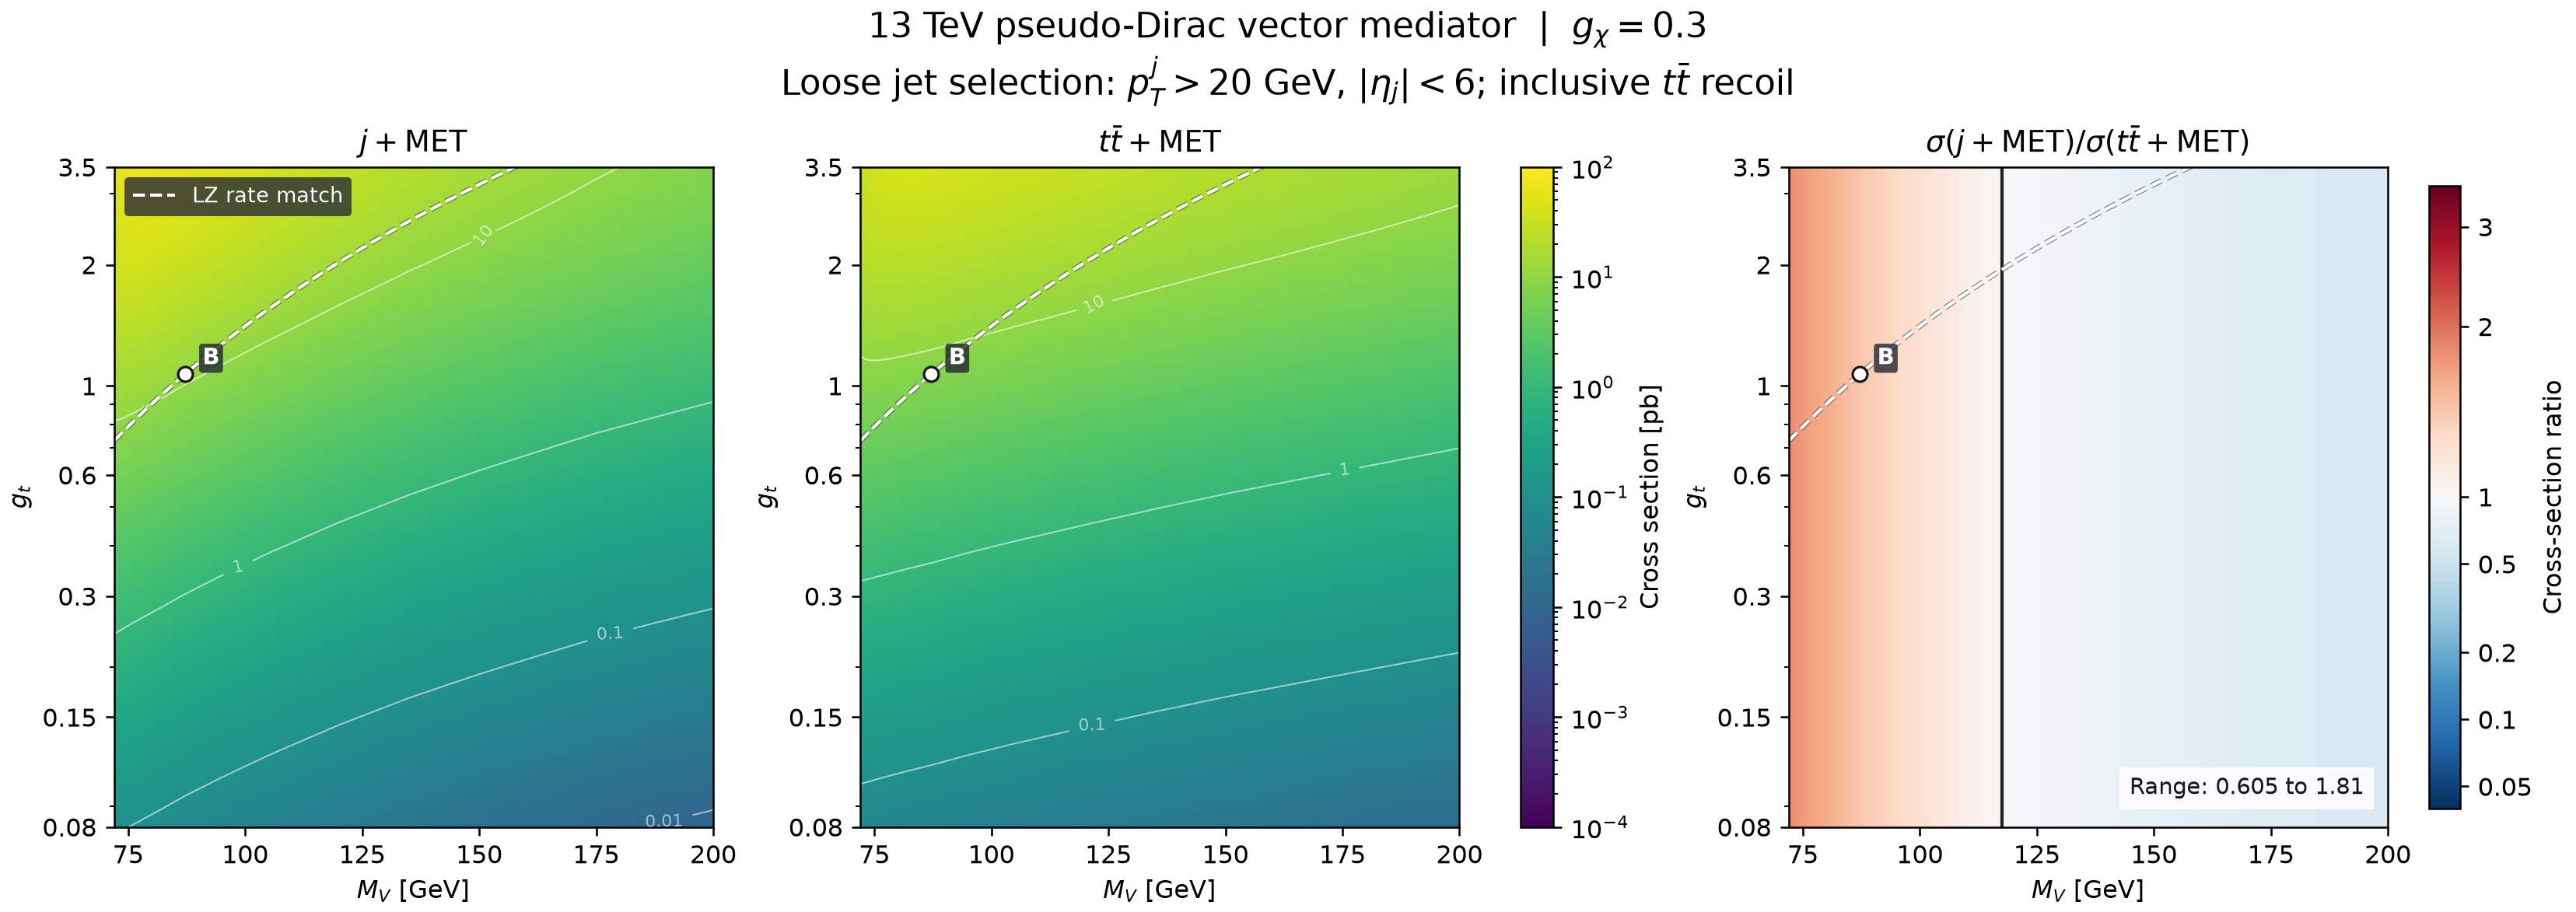
\includegraphics[width=.86\linewidth]{figures/b01_loose_cross_sections.png}
\caption{The jet selection is $p_T^j>20$ GeV and $|\eta_j|<6$, and the top-pair final state has no truth MET cut. Comparison with Fig.~\ref{fig:hard_met} shows the effect of the selection threshold.}
\label{fig:loose}
\end{figure}

\begin{figure}[tbp]
\centering
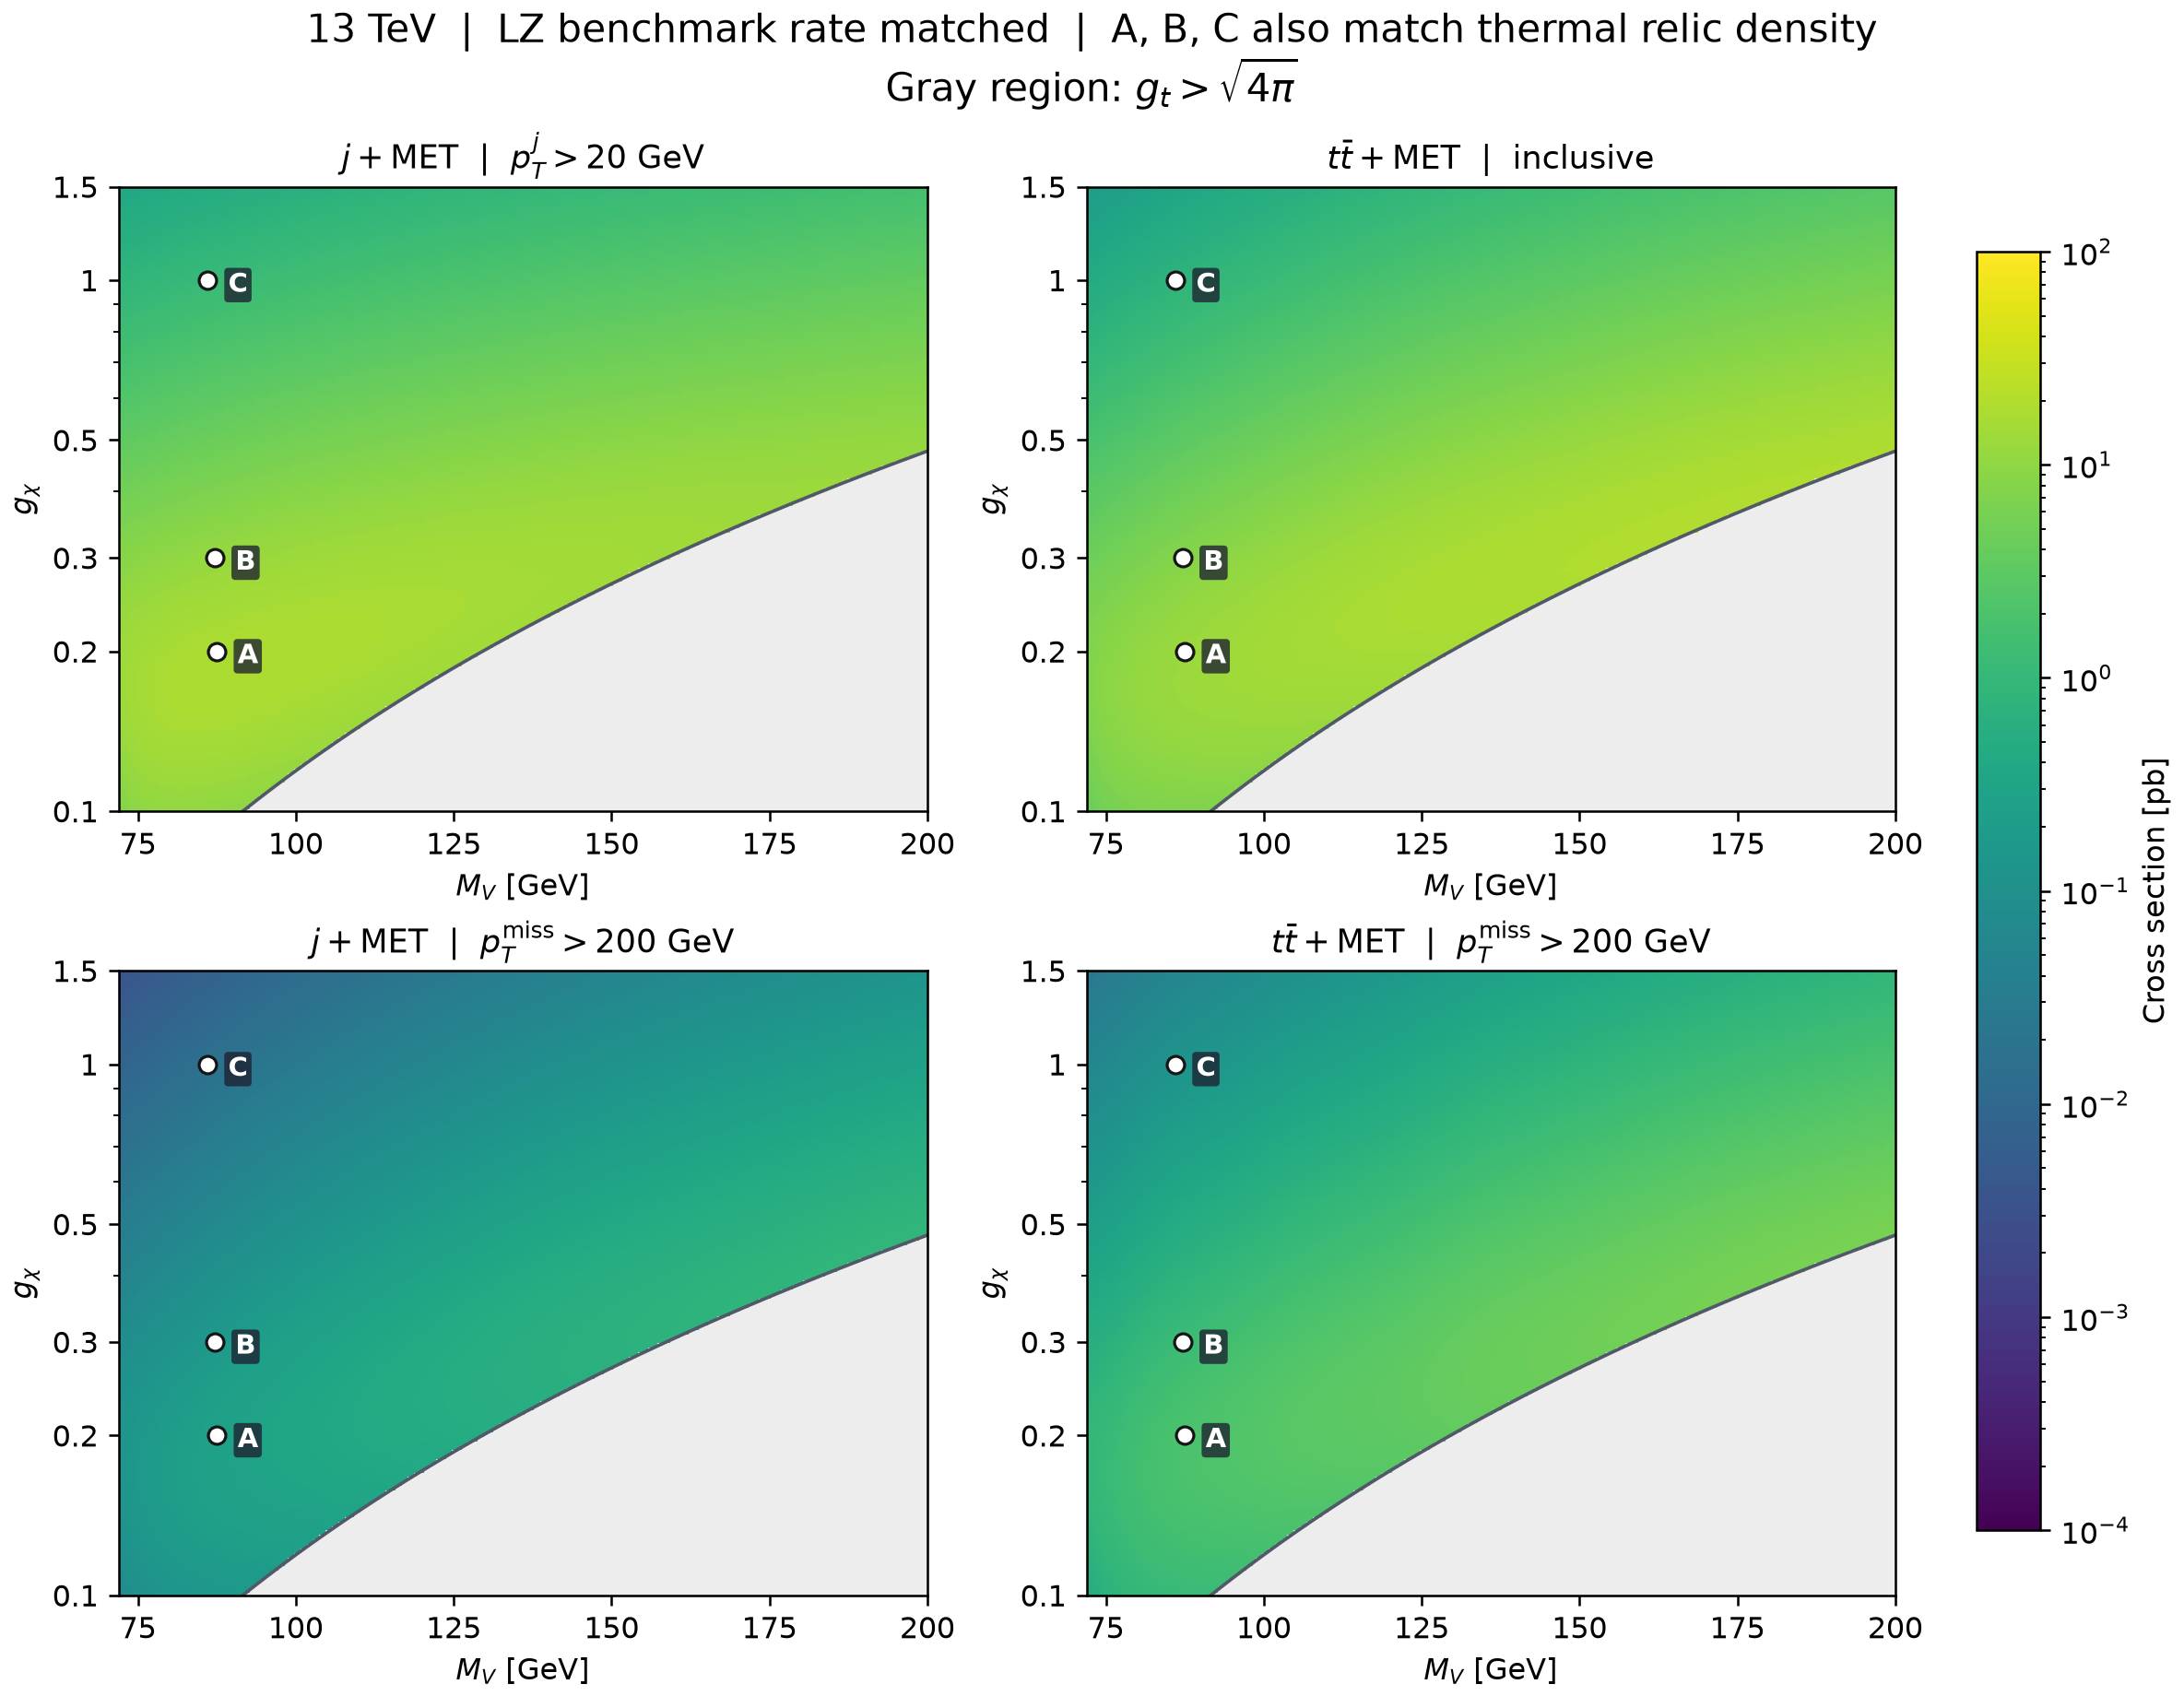
\includegraphics[width=.86\linewidth]{figures/b02_lz_slice_cross_sections.png}
\caption{We fix $m_\chi=35$ GeV and determine $g_t$ from the tree-level equal-rate condition. A, B, and C are separate relic-density benchmarks. The remaining colors show cross sections subject to the equal-rate condition alone.}
\label{fig:equal_rate_xsec}
\end{figure}

\begin{figure}[tbp]
\centering
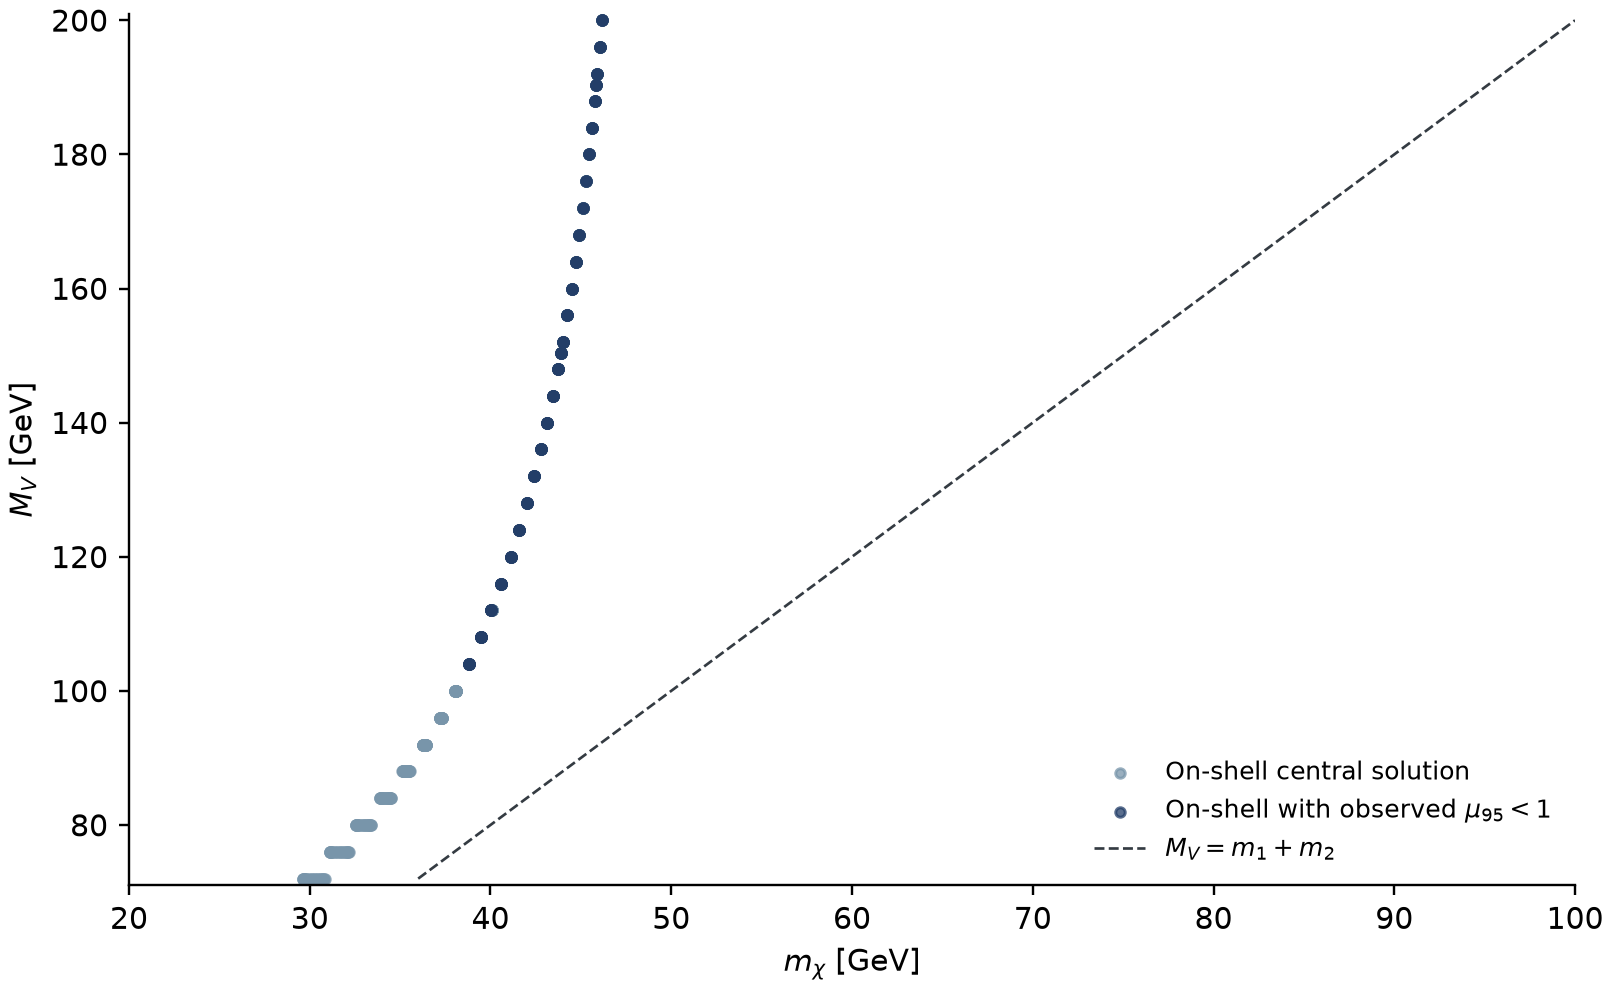
\includegraphics[width=.58\linewidth]{figures/04b_central_mass_projection.png}
\caption{Projection of the central relic grid onto $(m_\chi,M_V)$. Dark blue marks on-shell roots with observed $\mu_{95}<1$. Multiple coupling solutions can overlap in the mass projection.}
\label{fig:mass_projection}
\end{figure}

\section{Validation of the CMS monojet recast}
\label{sec:validation}

\begin{figure}[tbp]
\centering
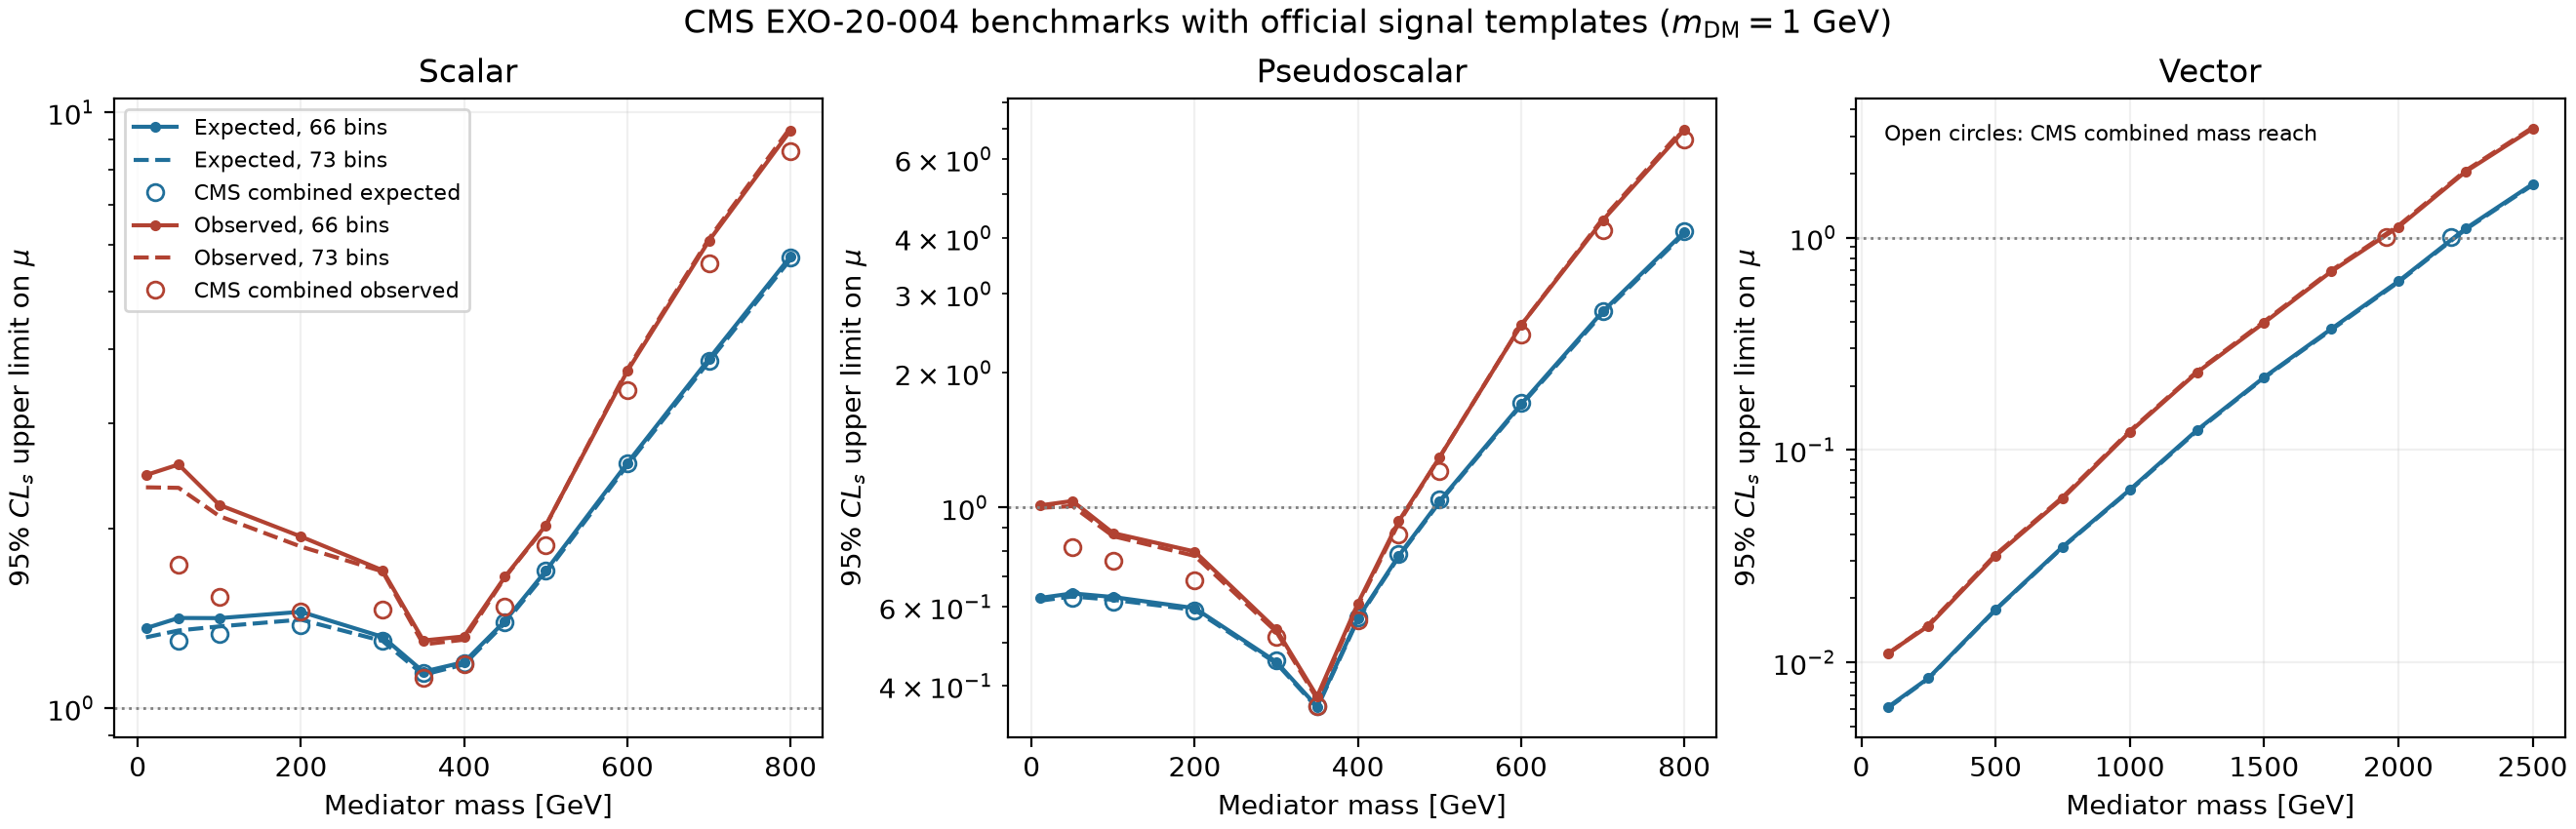
\includegraphics[width=.86\linewidth]{figures/c01_cms_benchmark_limits.png}
\caption{Comparison of limits obtained using official CMS signal templates. For scalar and pseudoscalar benchmarks between 50 and 800 GeV, the expected limits from the 66-bin fit differ from the published combination by at most about $9\%$. The largest difference in observed limits is about $48\%$. The mass boundaries provide a separate check of the overall reach for the official vector benchmark. \cite{cmsmonojet,cmssignal}}
\label{fig:cms_official}
\end{figure}

\begin{figure}[tbp]
\centering
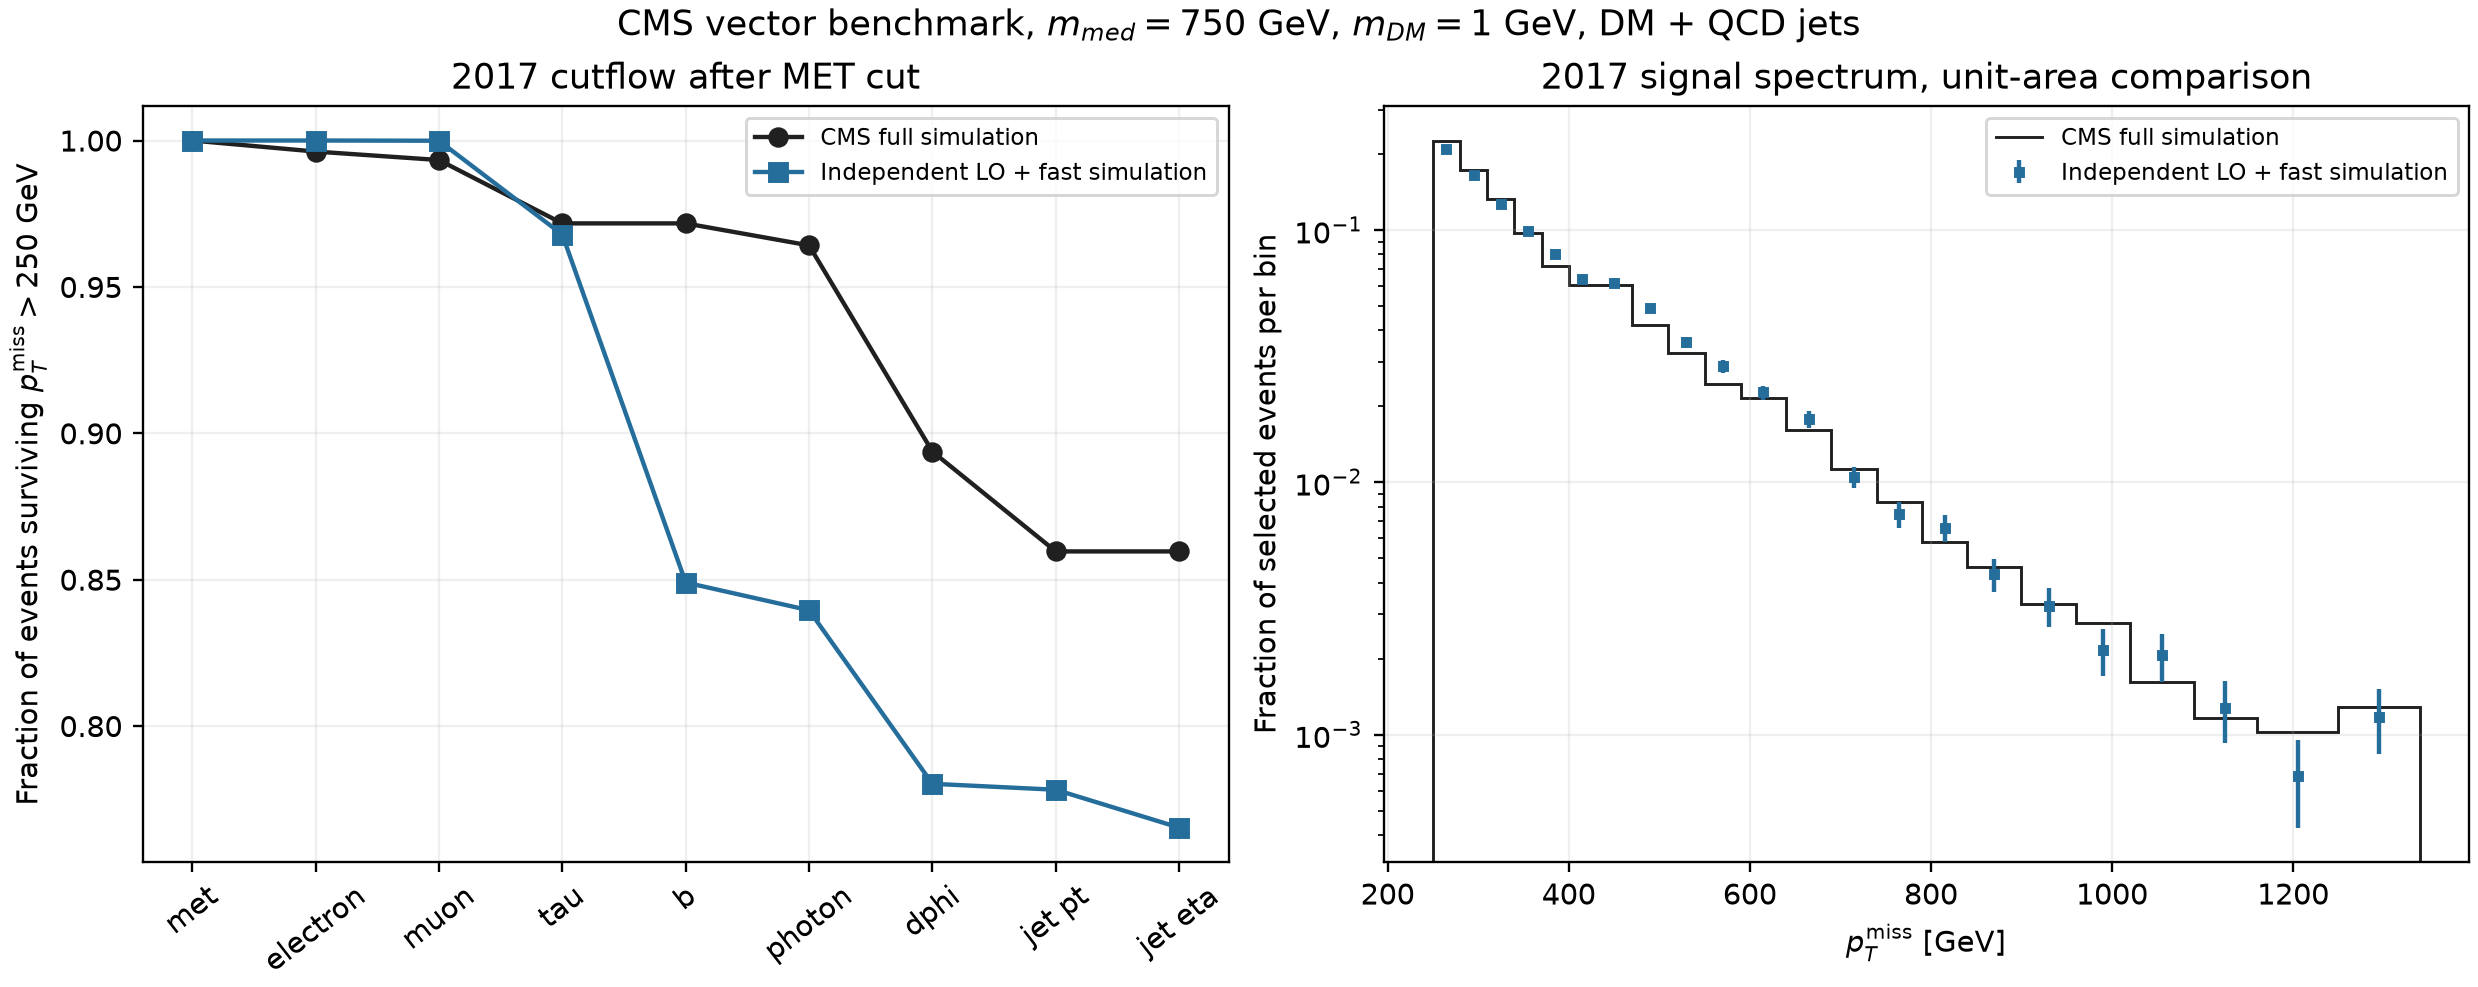
\includegraphics[width=.86\linewidth]{figures/c02_cms_vector_750.png}
\caption{Cutflow and MET spectrum for the 750 GeV CMS vector benchmark.}
\label{fig:cms_750}
\end{figure}

\begin{figure}[tbp]
\centering
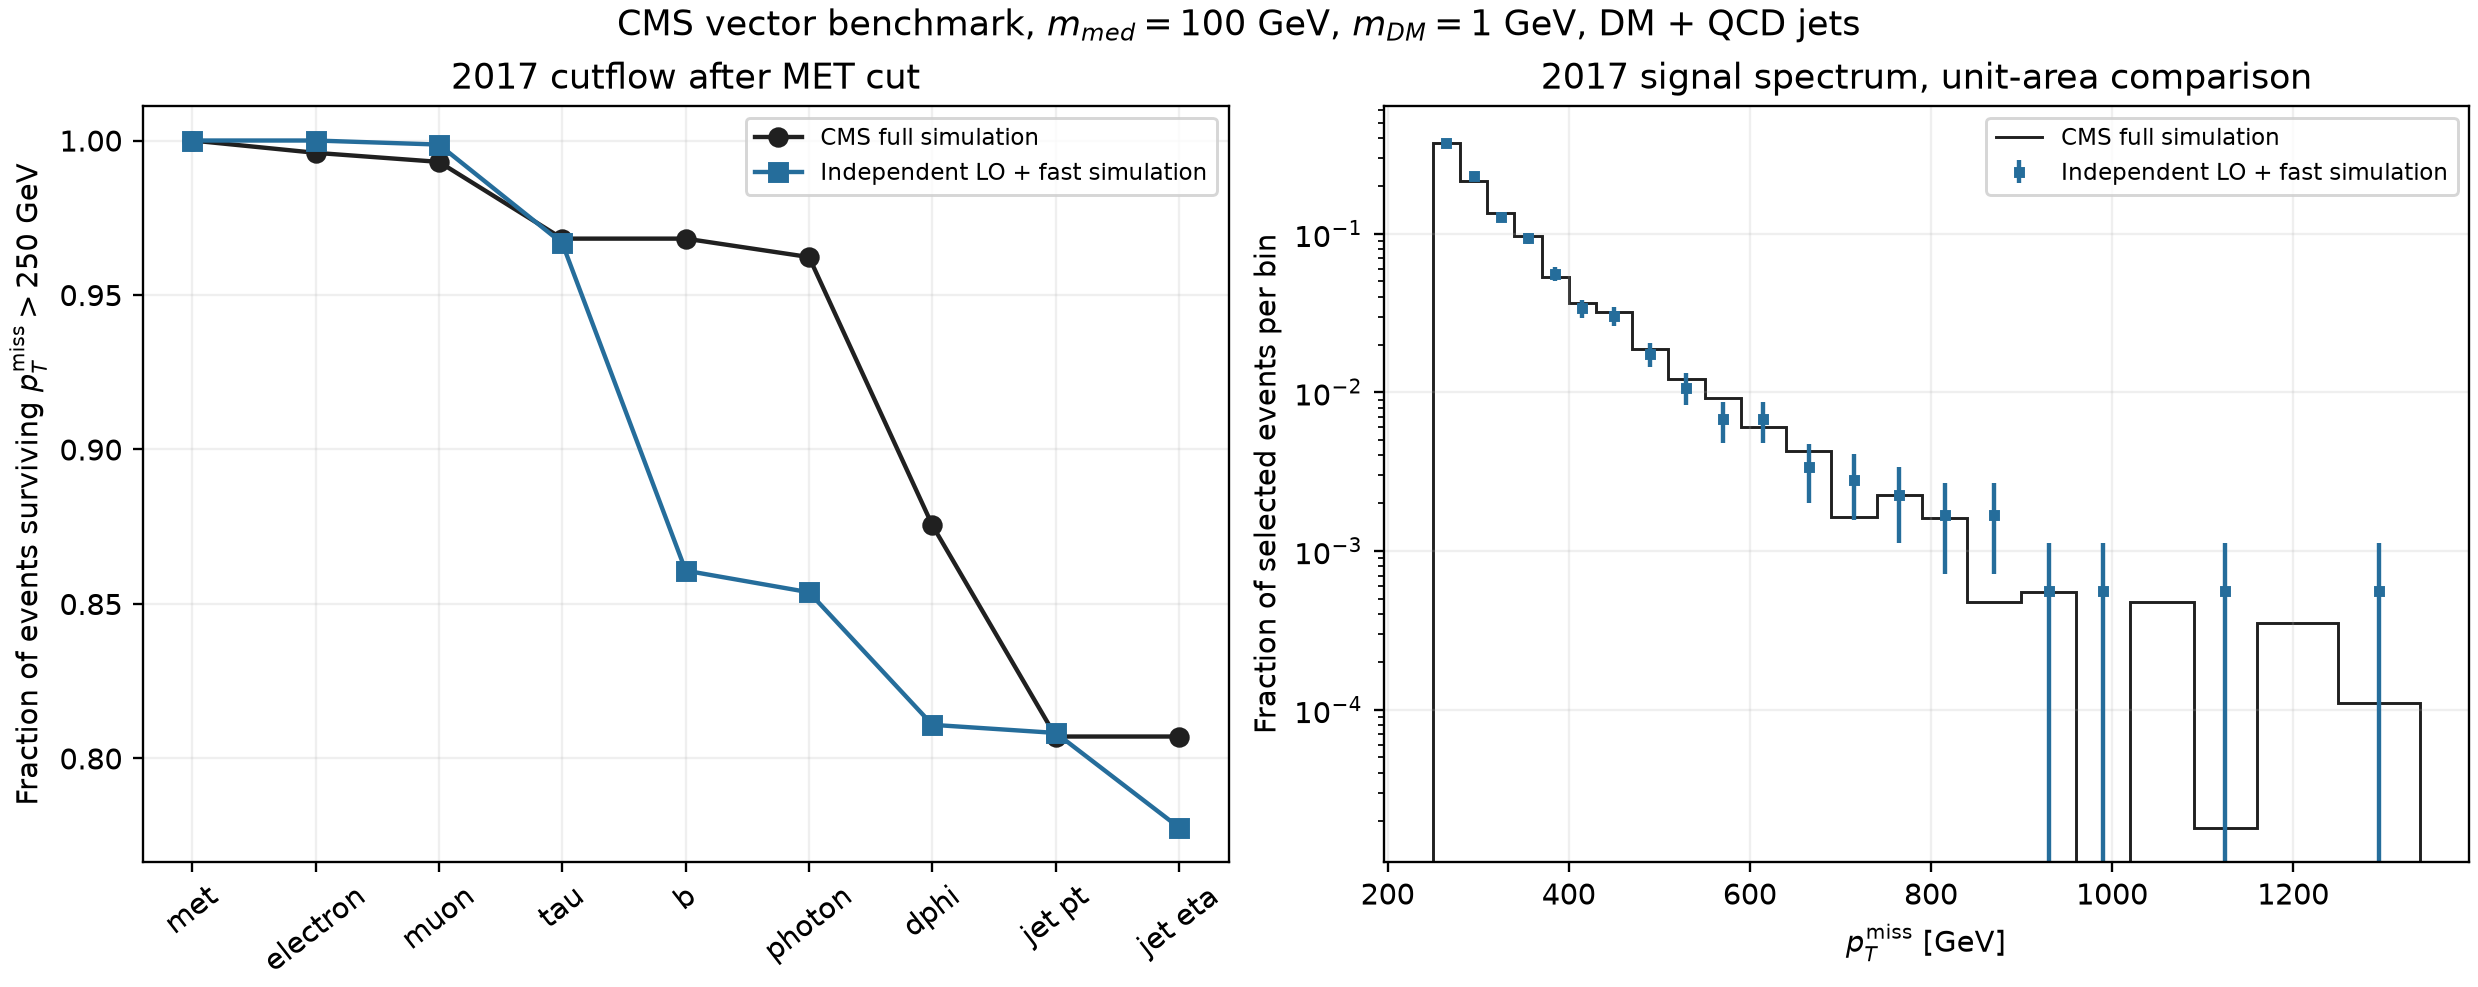
\includegraphics[width=.86\linewidth]{figures/c03_cms_vector_100.png}
\caption{Cutflow and MET spectrum for the 100 GeV CMS vector benchmark. Comparison of independent LO event generation and fast detector simulation with official CMS vector benchmarks. For the 100 GeV benchmark in 2017, the efficiency after the MET cut is $76.91\%$ for CMS and $77.76\%$ in our simulation. The absolute QCD signal yield in our simulation is 0.629 times the CMS yield. The two samples use different generator and reconstruction settings, including NLO matching in the official sample. We compare the normalized shapes and the absolute yields separately. \cite{cmscutflow}}
\label{fig:cms_100}
\end{figure}

\begin{figure}[tbp]
\centering
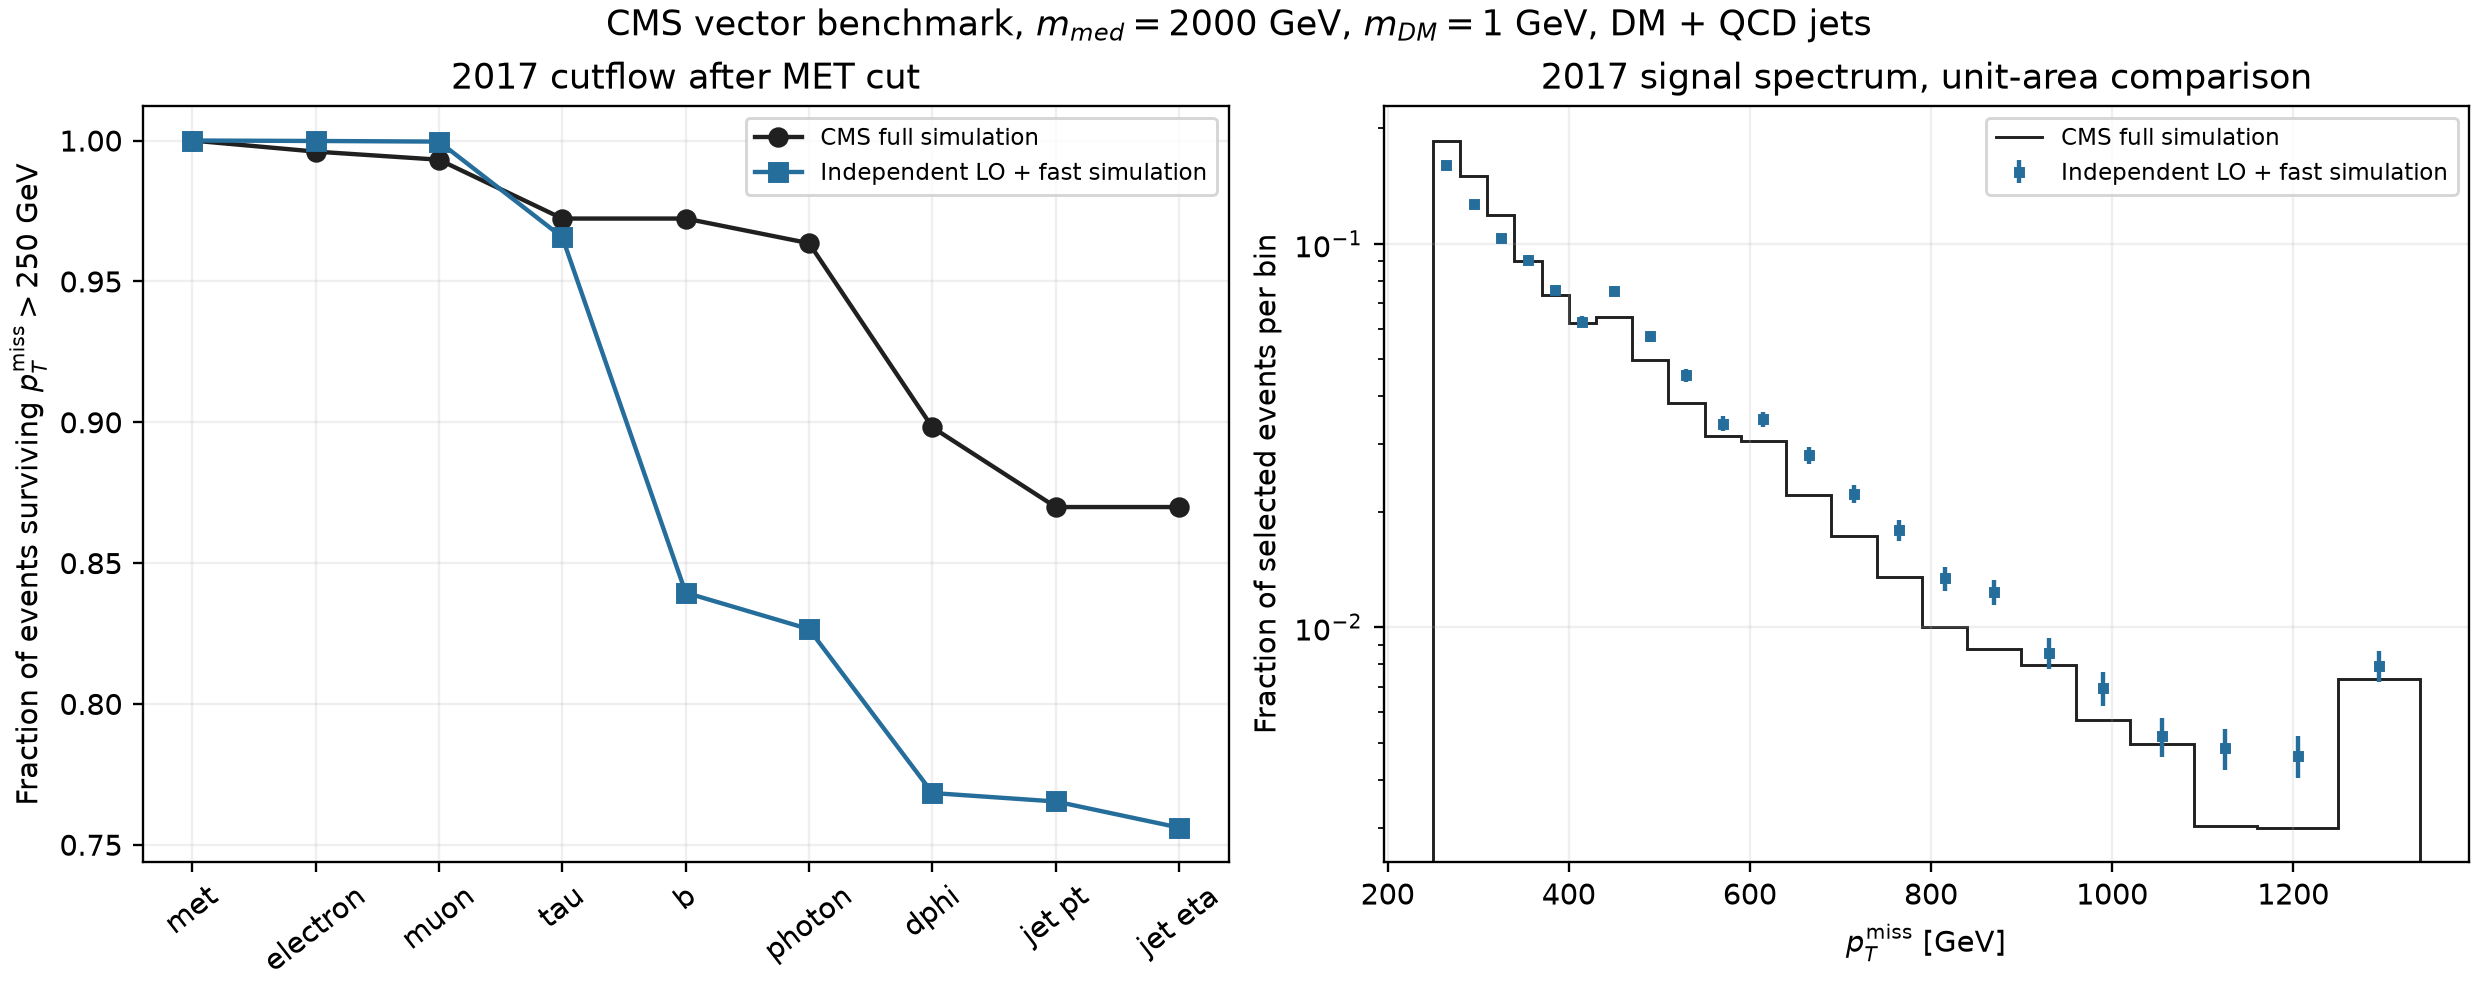
\includegraphics[width=.86\linewidth]{figures/c04_cms_vector_2000.png}
\caption{Cutflow and MET spectrum for the 2000 GeV CMS vector benchmark.}
\label{fig:cms_2000}
\end{figure}

\begin{figure}[tbp]
\centering
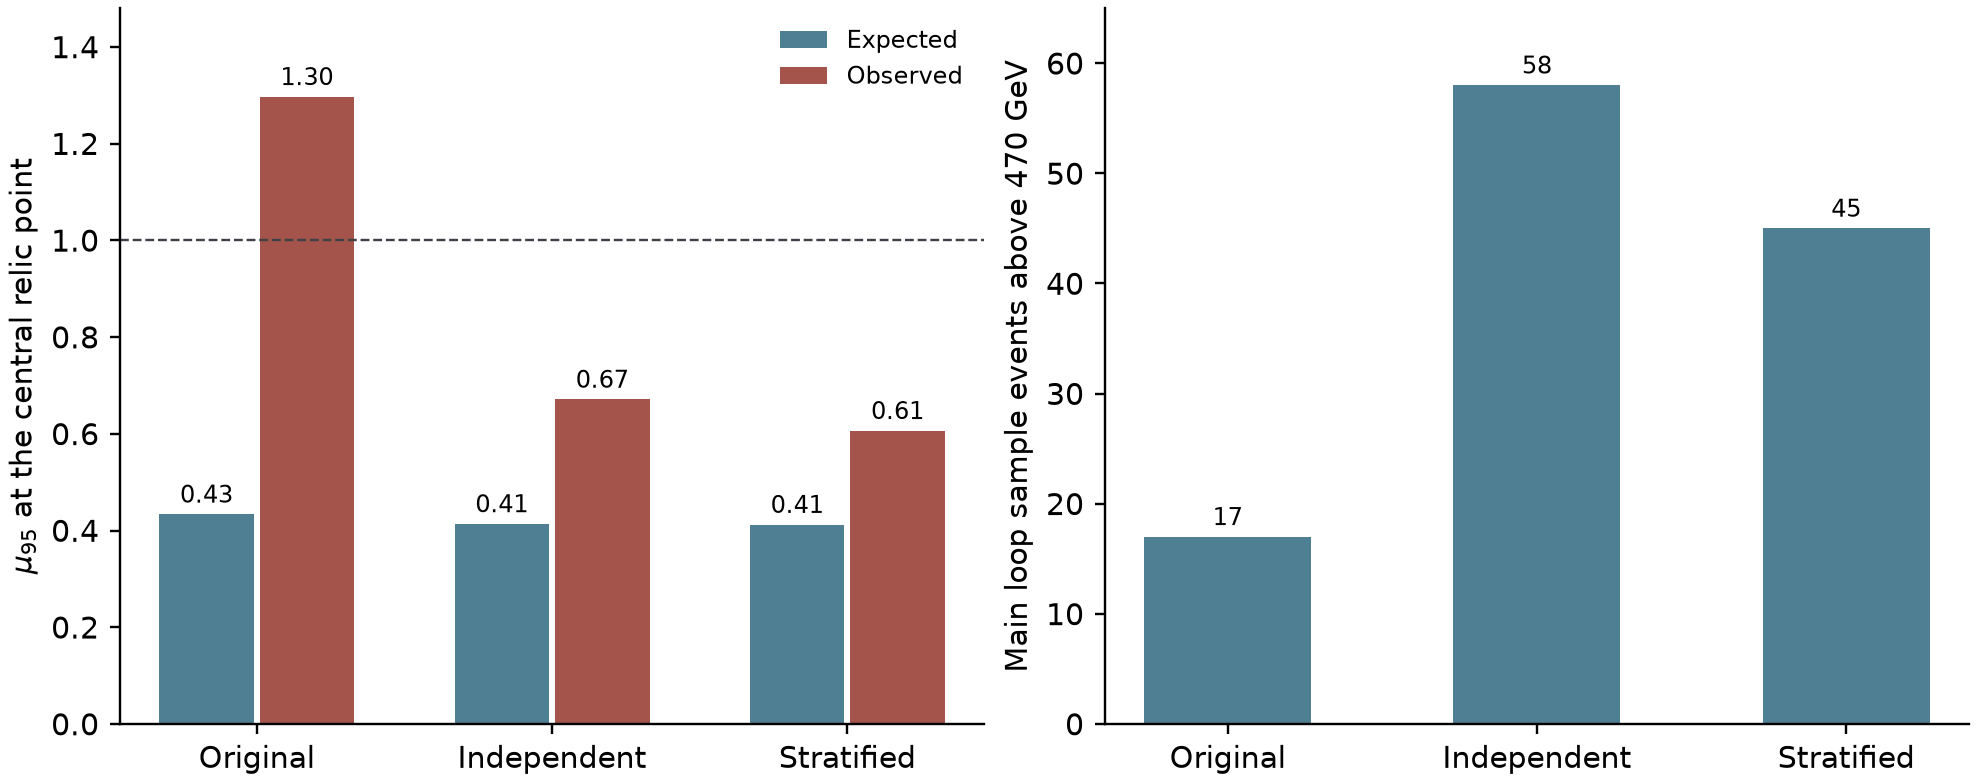
\includegraphics[width=.58\linewidth]{figures/c05_loop_mc_validation.png}
\caption{Of the 3,600 events in the original loop sample, 17 pass the reconstructed selection and fall in MET bins above 470 GeV. At the same central relic solution, the original sample gives an observed $\mu_{95}$ of about 1.30. An independent sample gives 0.67, and a stratified sample gives 0.61. The main analysis uses the stratified template and all observed counts.}
\label{fig:small_sample}
\end{figure}

\subsection{Independent template test at three sensitive benchmarks}

We keep $(M_V,g_t,m_\chi,g_\chi)$ fixed at the 120, 150.4, and 190.4 GeV benchmarks in Table~\ref{tab:benchmarks}, along with the 66-bin CMS likelihood and background covariance. Loop templates A and B use independent hard-process and shower samples, with generator-level jet $p_T$ boundaries of $(100,230,480)$ and $(100,260,520)$ GeV, respectively. The three strata typically contain 6,600, 4,000, and 3,200 generated events. For the lowest stratum of A at 120 and 150.4 GeV, we use an independent archived sample of 10,800 events and a new sample of 4,800 events, respectively, and retain events with $100\le p_T^j<230$ GeV. Both fits share a newly generated tree template. We also repeat both fits with the original tree template. We average the loop templates with equal weights, combine the Monte Carlo covariances with squared weights, and count the common tree uncertainty once.

We rank the year-specific MET bins using $|s_i[(C_b+\operatorname{diag}\mathbf b)^{-1}\mathbf s]_i|$, evaluated with the reference signal and the background-only information. In the eight highest-ranked bins, we compare the yield differences with the Monte Carlo uncertainties of the independent loop samples. We also sum yields across years in the 470--690 GeV and above-690 GeV intervals and refit the upper limits using all 66 bins.

\begin{table}[tbp]
\caption{Comparison of independent signal templates for the three sensitive benchmarks. The final column gives the largest discrepancy in one of the eight key bins in units of the Monte Carlo (MC) uncertainty.}
\label{tab:templates}
\begin{ruledtabular}
\begin{tabular}{rccc}
$M_V$ [GeV] & Expected A / B / pooled & Observed A / B / pooled & Max. difference ($\sigma_{\rm MC}$) \\
\hline
120 & 0.389 / 0.407 / 0.408 & 0.527 / 0.621 / 0.561 & 1.05 \\
150.4 & 0.230 / 0.243 / 0.242 & 0.219 / 0.254 / 0.234 & 0.88 \\
190.4 & 0.174 / 0.178 / 0.179 & 0.200 / 0.200 / 0.198 & 1.68 \\
\end{tabular}
\end{ruledtabular}
\end{table}

\begin{figure}[tbp]
\centering
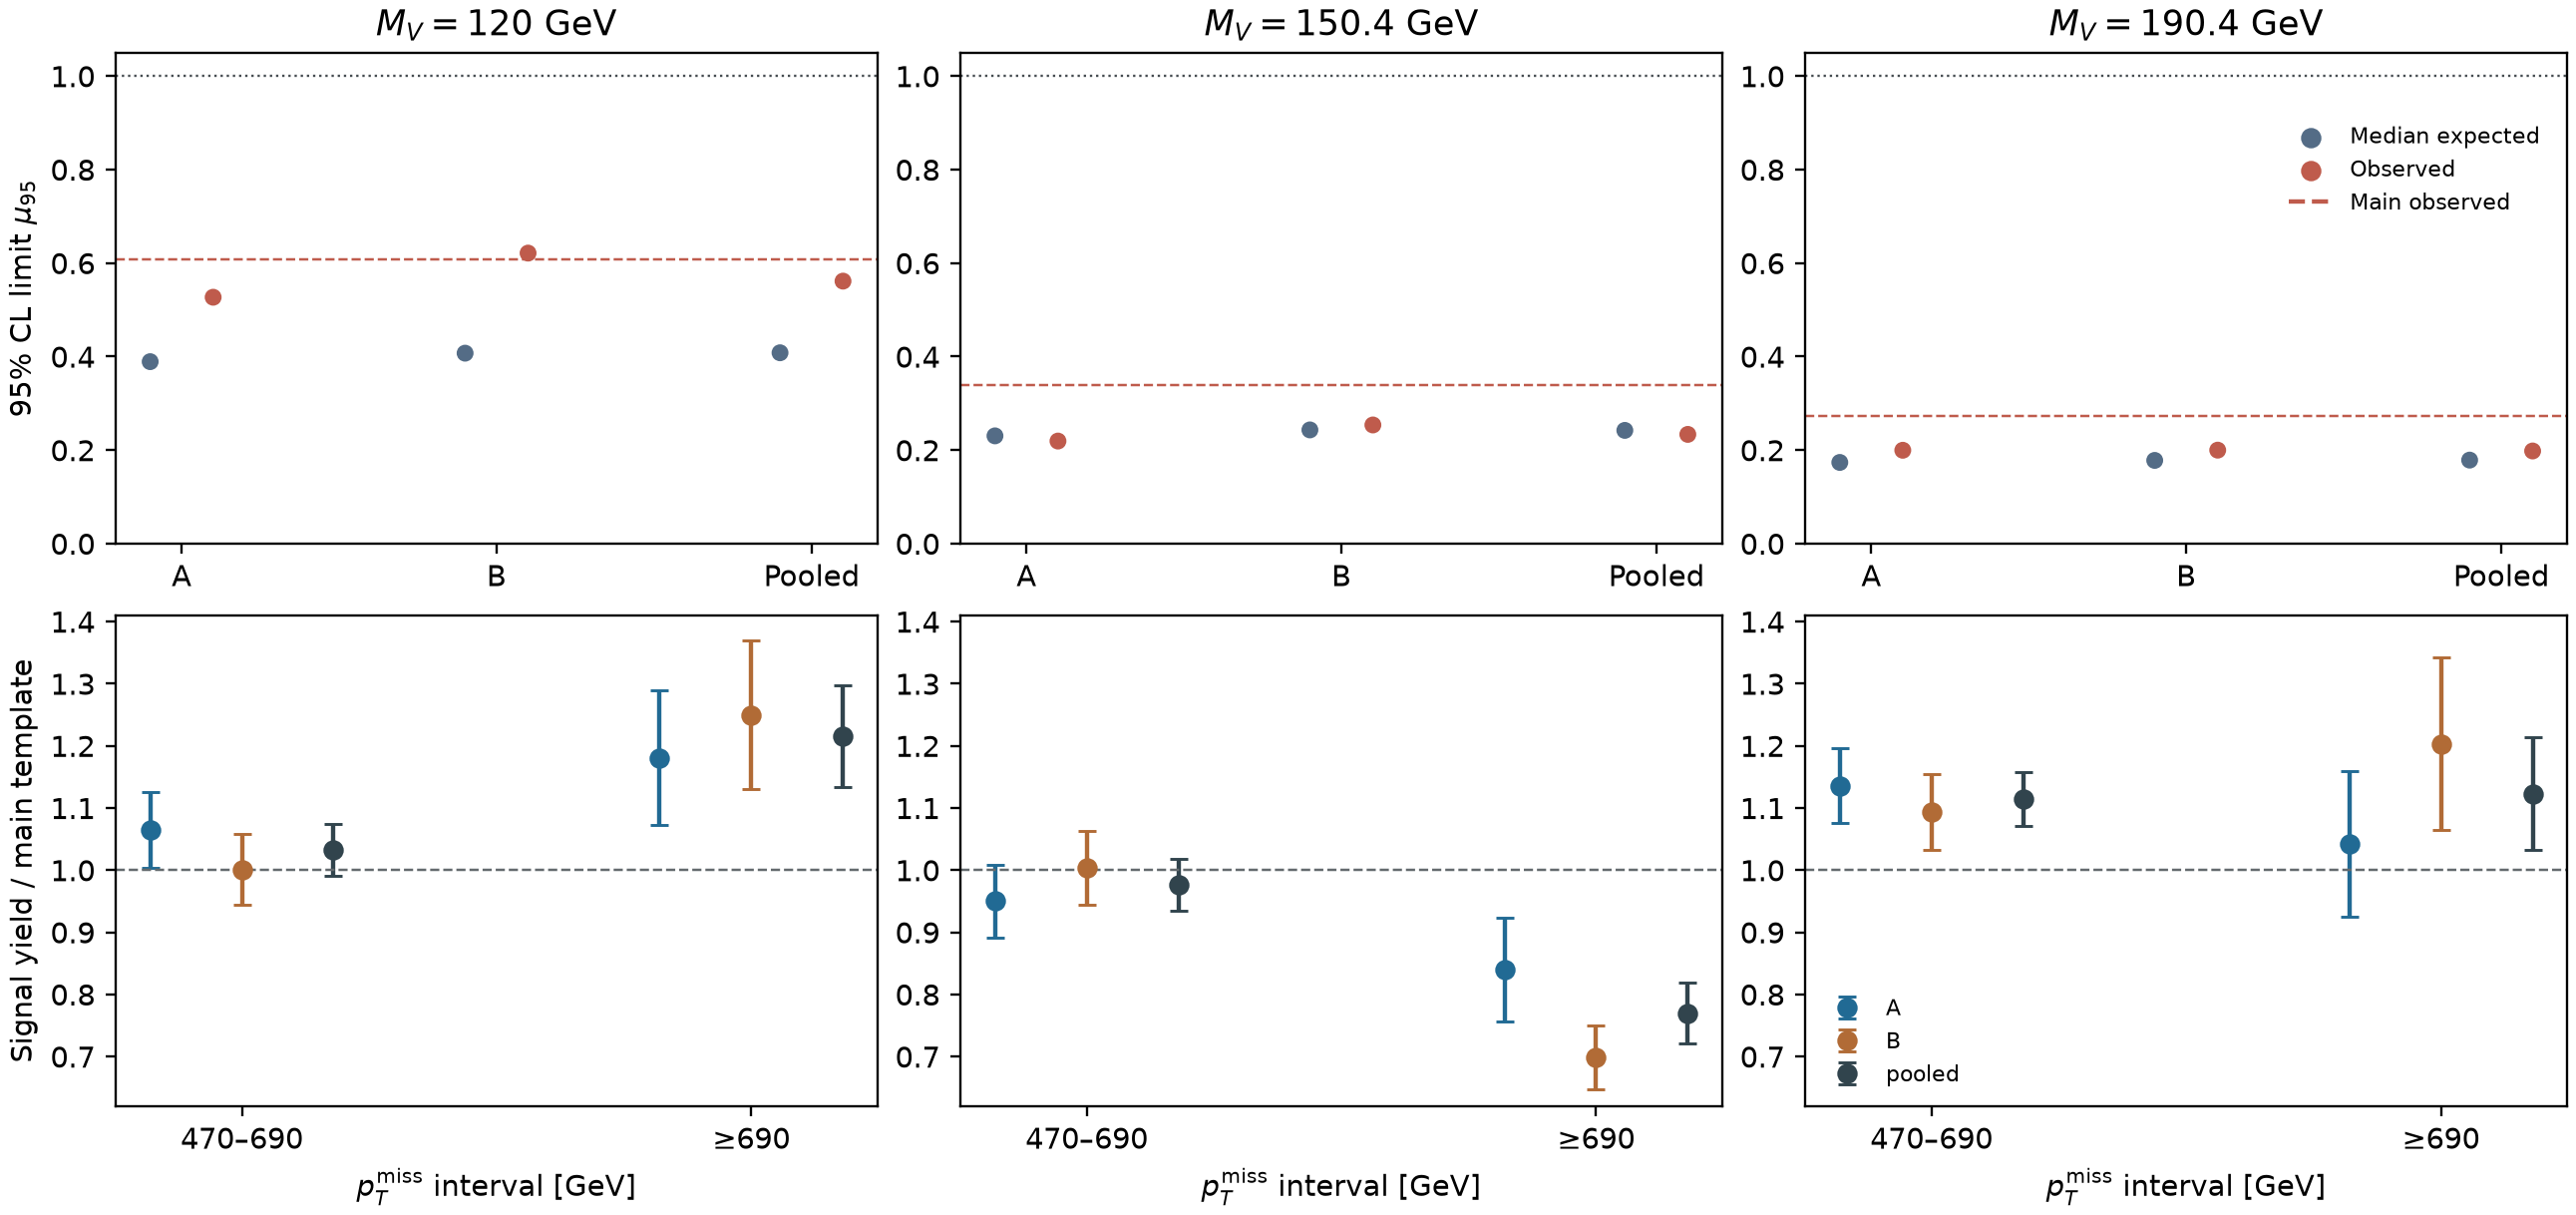
\includegraphics[width=.86\linewidth]{figures/c06_three_template_replicas.png}
\caption{The top panels show the CMS 95\% CL limits. The dashed lines mark the reference observed limits from Table~\ref{tab:benchmarks}. The lower panels show the yield of each template divided by the reference yield in two combined MET intervals. The error bars represent the Monte Carlo uncertainty of each template. The accompanying analysis tables give yields by year and bin.}
\label{fig:independent_samples}
\end{figure}

The two templates agree within about $1.7$ Monte Carlo standard deviations in the key bins and combined high-MET intervals. All three benchmarks give observed $\mu_{95}<1$. Across templates and target yields in the range $r=0.75$--$1.25$, the largest observed limit is $0.680$. At 120 and 150.4 GeV, the two stratifications still give observed limits that differ by about $16\%$ and $15\%$ of their mean, respectively. At 150.4 and 190.4 GeV, the pooled limits are about $31\%$ and $27\%$ below the reference values in Table~\ref{tab:benchmarks}. The three exclusion decisions are stable across the sampling schemes tested, while the numerical limits retain some dependence on Monte Carlo statistics and template shape.

We refit the original grid with the three pooled templates, replacing the 120 and 150 GeV nodes and adding the 190.4 GeV node. After interpolation, the number of points with expected $\mu_{95}<1$ changes from 208 to 199, and the observed count changes from 151 to 162. The lowest sampled masses remain 92 and 104 GeV, respectively. The absolute yield discrepancy in Fig.~\ref{fig:cms_100} still limits the validation of the signal acceptance.

\section{Top-associated channels for light mediators}
\label{sec:top}

\subsection{Top-pair production}

With the loose jet cut $p_T^j>20$ GeV, the truth-level $j+\mathrm{MET}$ cross section is comparable to the inclusive $t\bar t+\mathrm{MET}$ cross section near $M_V\simeq118$ GeV. Applying $p_T^{\rm miss}>200$ GeV to both channels gives a cross-section ratio $\sigma(j+\mathrm{MET})/\sigma(t\bar t+\mathrm{MET})$ of $0.135$--$0.149$. For example, at $(m_\chi,M_V,g_t,g_\chi)=(35,87.18,1.070,0.30)$ the two cross sections are $0.166$ and $1.23$ pb, respectively. We treat the top quarks as stable, so $p_T^{\rm miss}=p_T(V)$. \cite{cox2016,alwall2014,hirschi2015}

\begin{figure}[tbp]
\centering
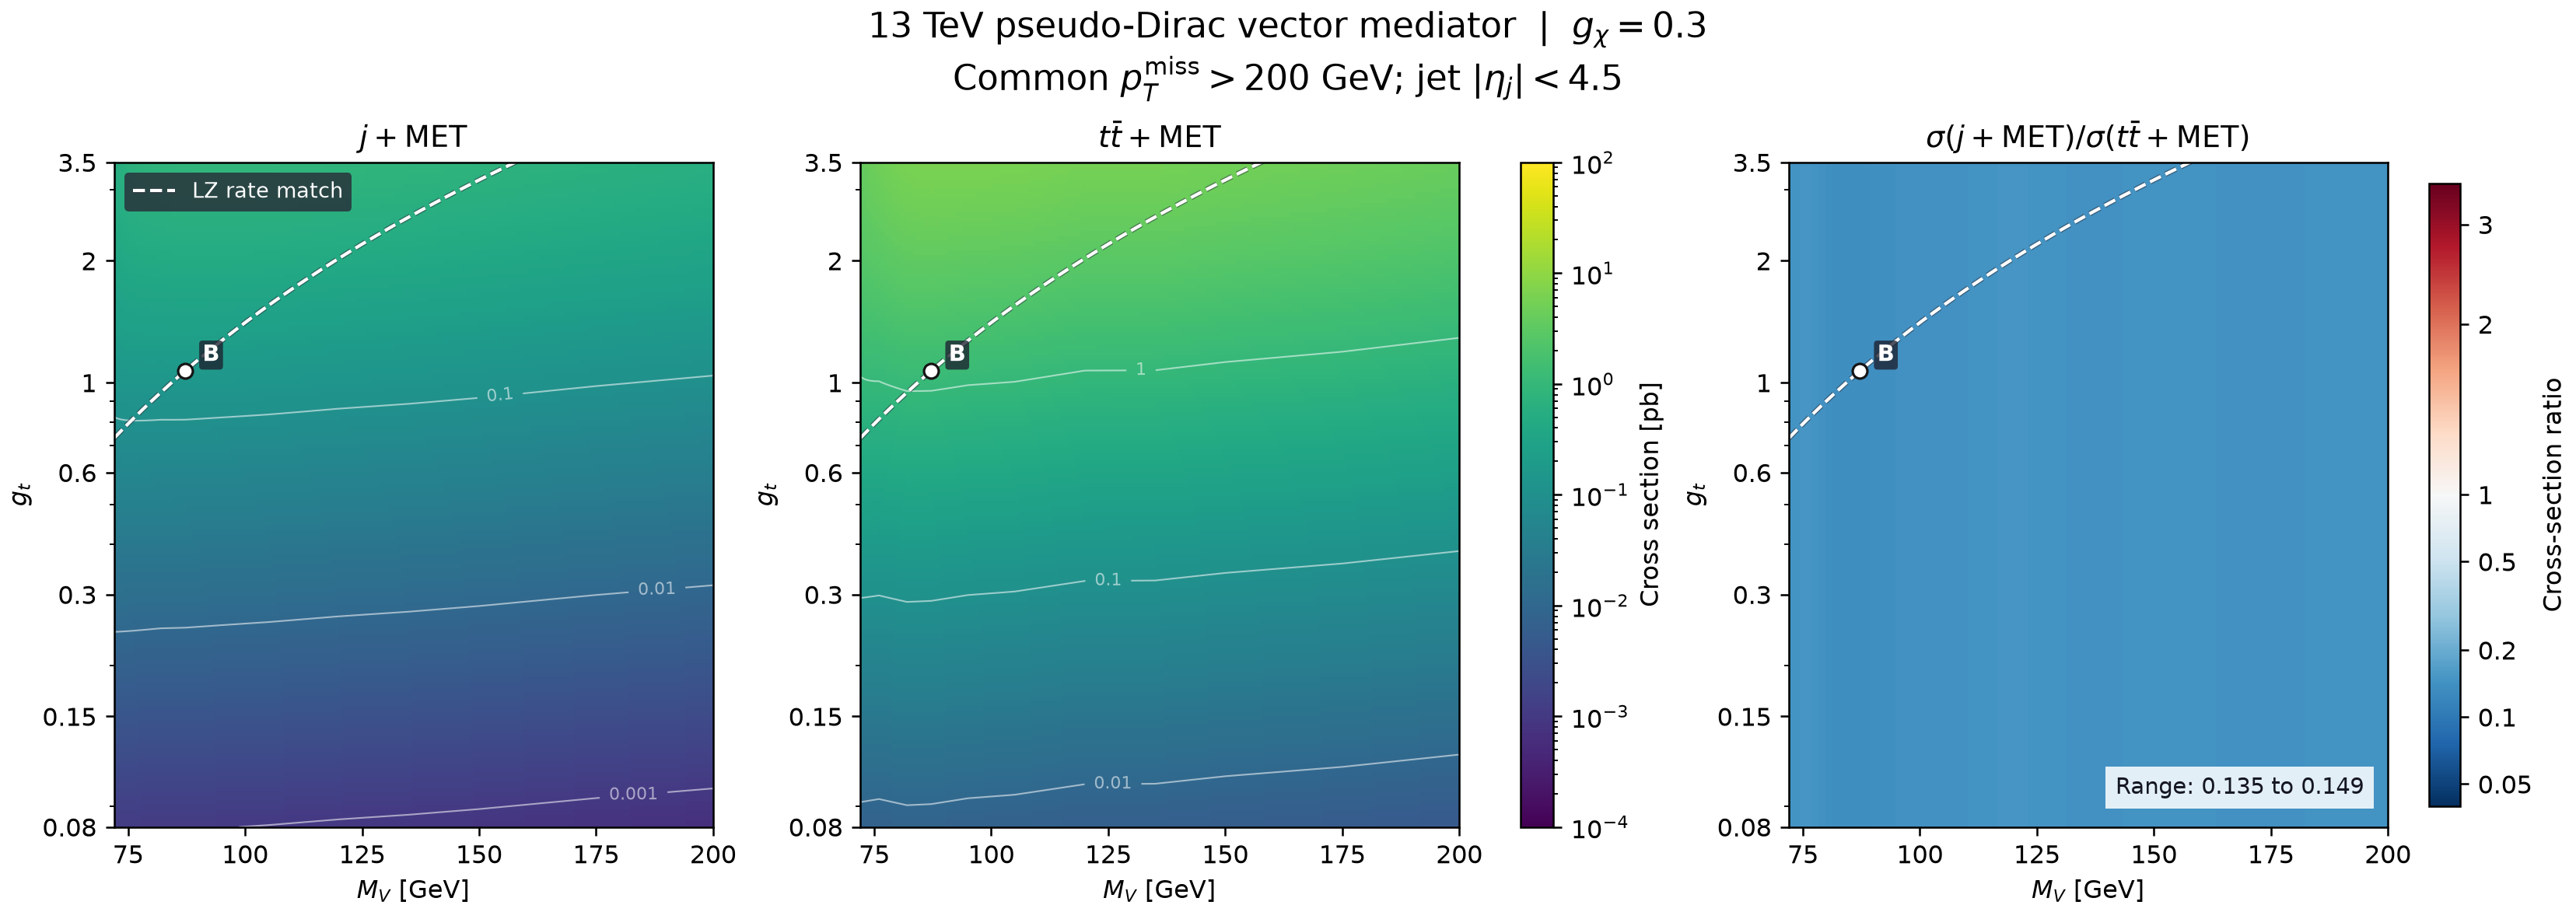
\includegraphics[width=.86\linewidth]{figures/03_hard_met_cross_sections.png}
\caption{Truth-level cross sections in pb and their ratio for $m_\chi=35$ GeV and $g_\chi=0.30$. The dashed curve shows the tree-level LZ yield-matching condition. The monojet cross section includes the leading tree channels and the $gg\to gV$ loop contribution.}
\label{fig:hard_met}
\end{figure}

The large top-quark coupling $g_t$ makes $pp\to t\bar tV^{(*)}\to t\bar t\chi_1\chi_2$ another possible collider probe. On-shell enhancement can occur when $M_V>2m_\chi+\Delta m$. Below this threshold we generate the four-body final state directly. In the low-mass scan, $(M_V,g_t)=(48\,\mathrm{GeV},0.252)$ has three solutions at the central abundance, with $m_\chi=20.445,25.260,45.878$ GeV. The lightest solution is on shell. At off-shell benchmarks with $M_V=30,46,60$ GeV, the full matrix element at 13 TeV gives $t\bar t+\mathrm{MET}$ cross sections of $0.033$, $0.041$, and $1.13$ fb, respectively, for truth-level $p_T^{\rm miss}>250$ GeV. Limits in the CMS all-hadronic two-$b$-tag category also require the acceptance after top decays, the binned signal yields, and the background correlations. \cite{cmstop}

\subsection{Single-top sensitivity}

For the single-top channel $pp\to tj\chi_1\chi_2$, we estimate the expected sensitivity in the 15 bins of the CMS AH $1b\,1\mathrm{FJ}$ category. We approximate the backgrounds with the published central values and bin uncertainties from the fit with a 100 GeV scalar signal, keeping only the diagonal covariance. For the signal we use truth-level cuts, simplified top decays, and approximate $b$ tagging. At $(M_V,g_t)=(60\,\mathrm{GeV},0.399)$, the cuts $\sqrt{\hat s}<1.5,1.0,0.75$ TeV give median expected limits of $0.052,0.337,3.43$, respectively. The strong dependence on this cut is related to the charged weak current connecting up- and down-type quarks with unequal vector couplings. We use the cut variation to test the contribution of high-energy events. A quantitative exclusion requires an electroweak completion and validation of the reconstructed signal and background constraints. \cite{kahlhoefer2016,cmstop,cmsahdata}

\begin{figure}[tbp]
\centering
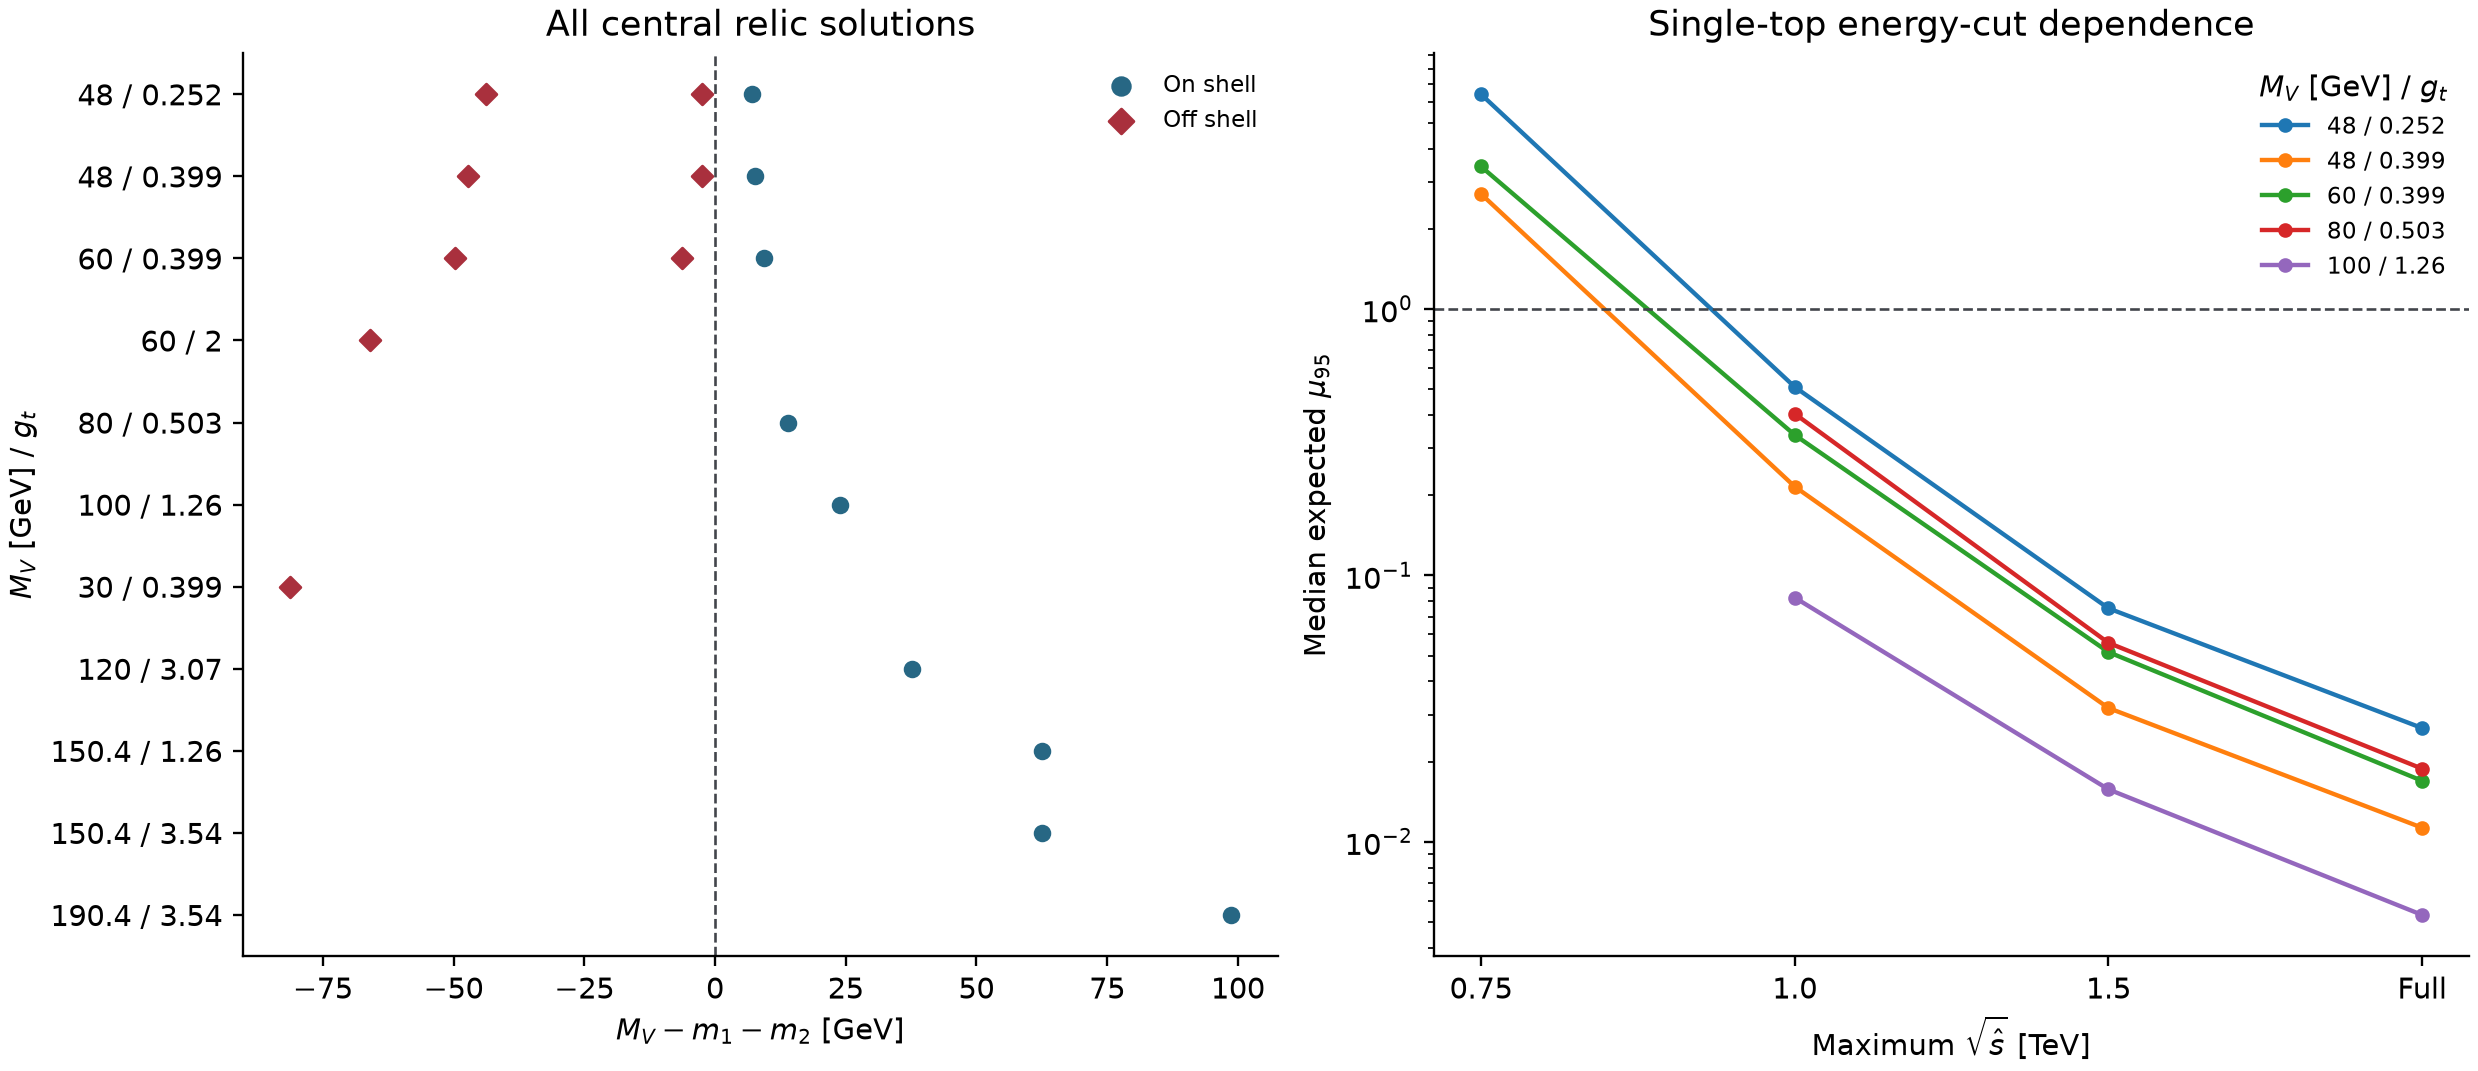
\includegraphics[width=.86\linewidth]{figures/08_top_branches_and_energy.png}
\caption{The left panel shows $M_V-m_1-m_2$ at representative central relic solutions. The right panel shows how the expected single-top sensitivity varies with the partonic-energy cut for on-shell solutions. The charged weak current connects top and bottom quarks with different $V$ couplings, so the high-energy behavior of longitudinal weak-boson amplitudes depends on cancellations in the electroweak completion. Varying the cut probes that dependence. Missing markers at 0.75 TeV indicate samples for which the approximate likelihood gives no finite limit.}
\label{fig:single_top_cut}
\end{figure}

\subsection{Low-mass branches and truth-level rates}

\begin{figure}[tbp]
\centering
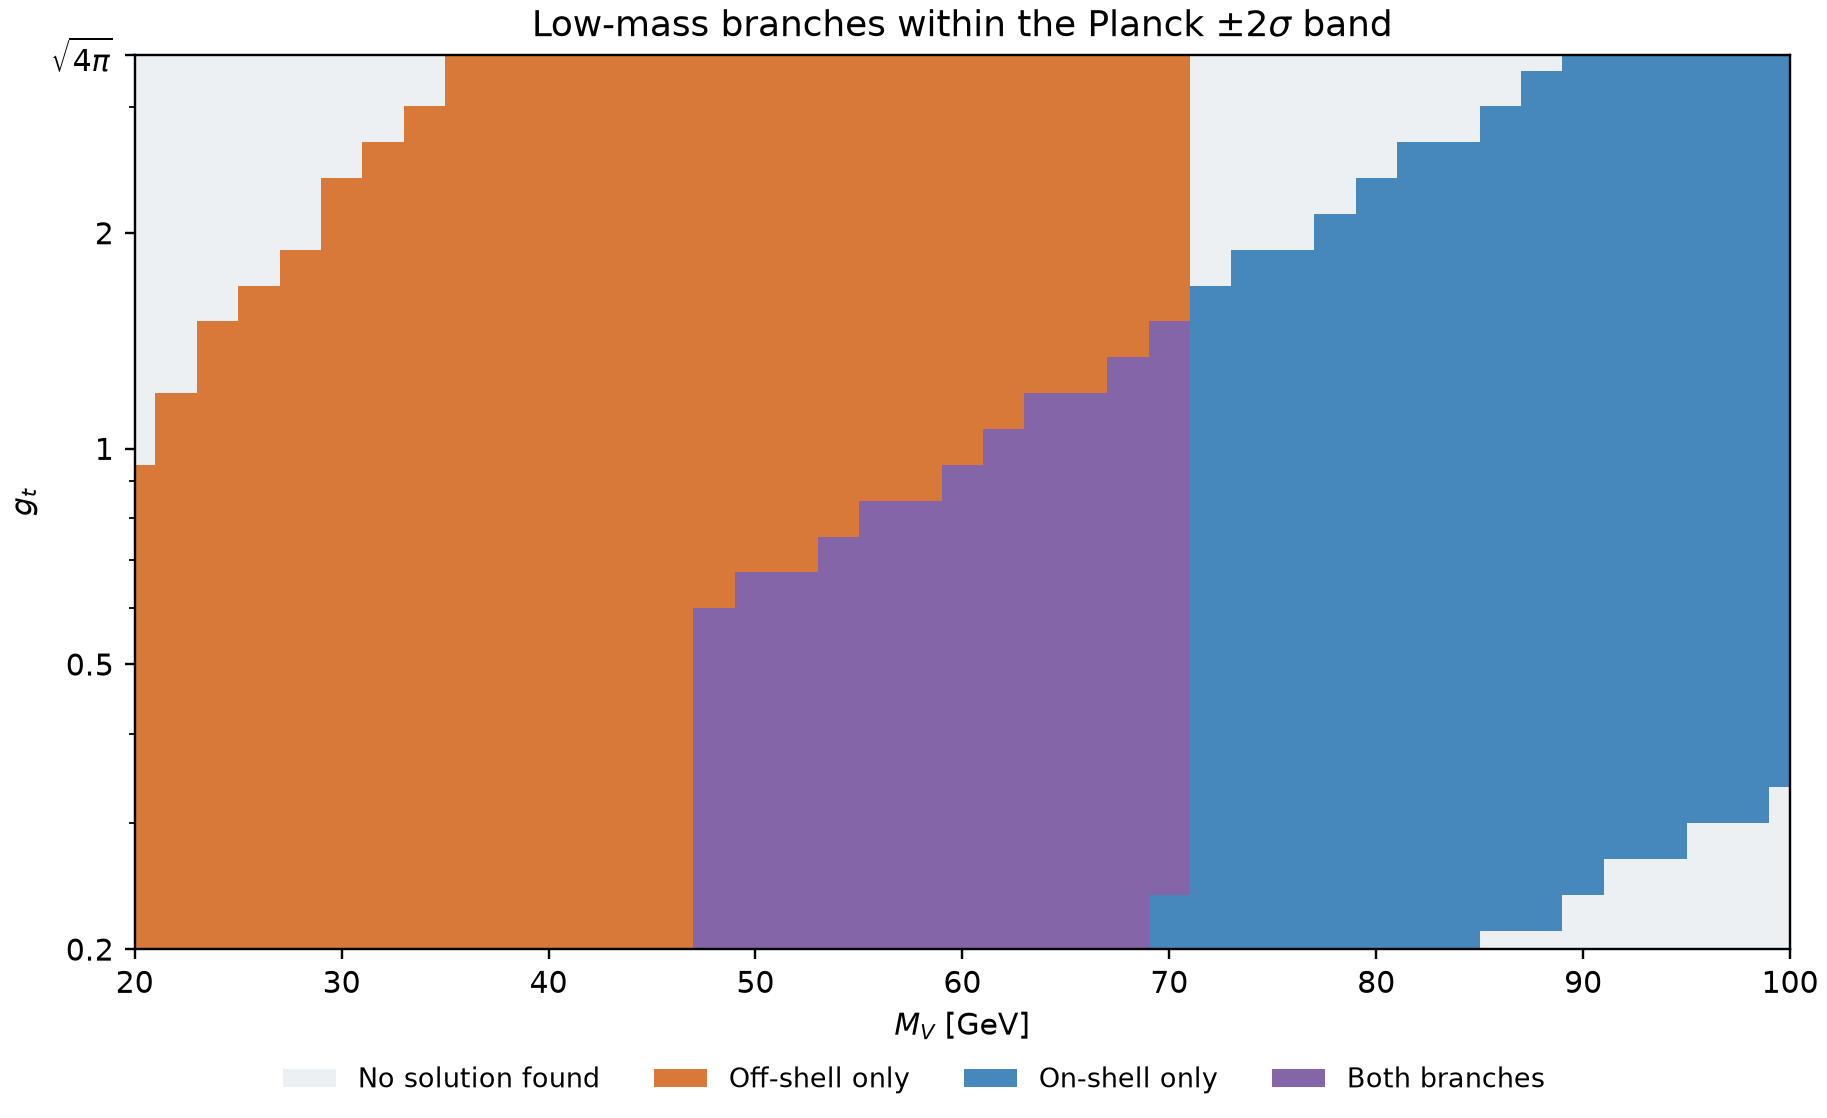
\includegraphics[width=.58\linewidth]{figures/d01_light_top_branches.png}
\caption{Independent low-mass scan with tree-level yield matching. Colors identify the relic branches found within the Planck $\pm2\sigma$ band. Purple indicates that both on-shell and off-shell solutions are present.}
\label{fig:low_mass}
\end{figure}

\begin{figure}[tbp]
\centering
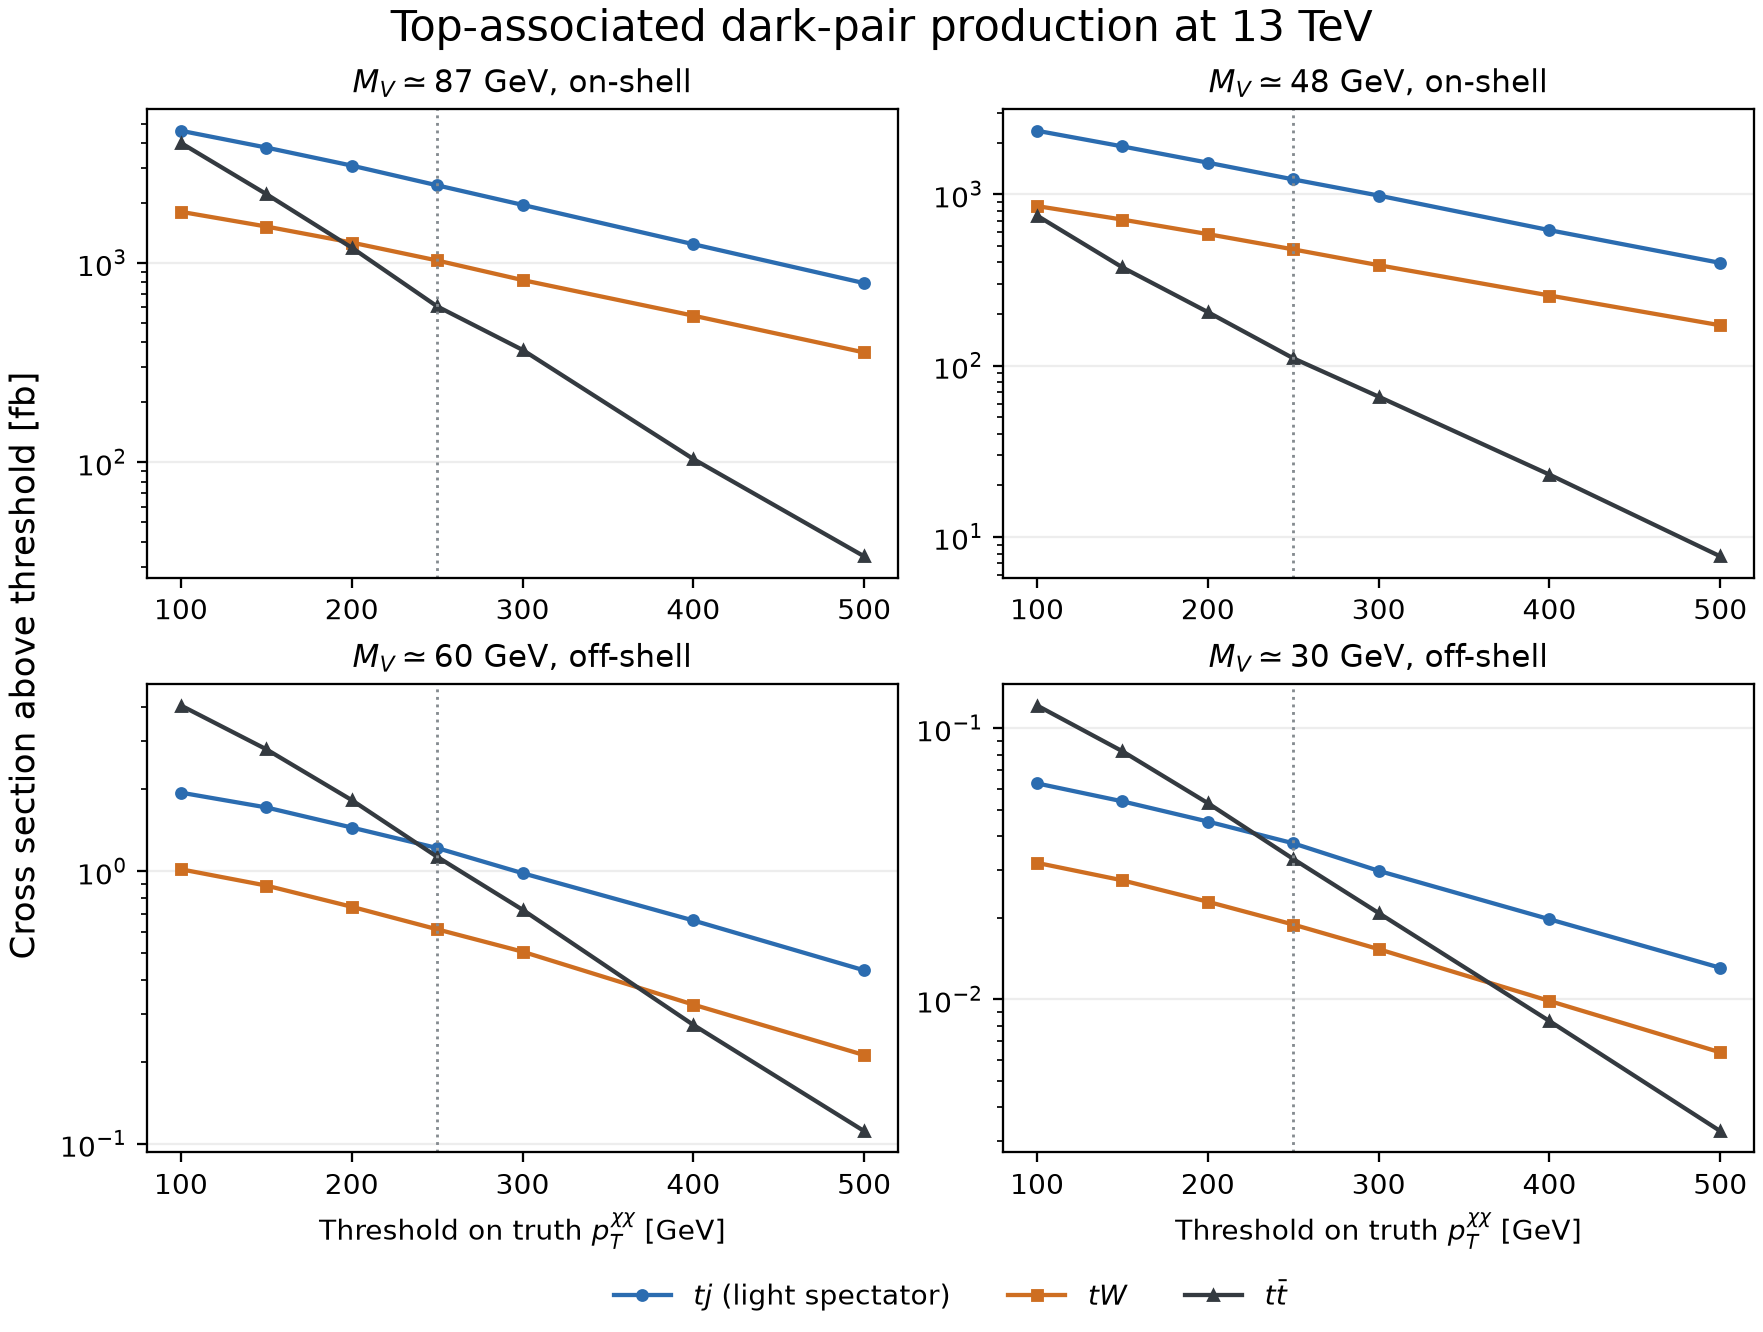
\includegraphics[width=.86\linewidth]{figures/d02_top_truth_met.png}
\caption{Cross sections in fb above different truth-level MET thresholds for dark-pair production with $tj$, $tW$, or $t\bar t$ at four on-shell or off-shell benchmarks. Deriving experimental limits requires simulating top decays and validating reconstruction and selection efficiencies at the same parameter points.}
\label{fig:top_truth_met}
\end{figure}

For $m_\chi\ge20$ GeV and $M_V\le40.001$ GeV, dark-pair production proceeds through an off-shell mediator. To derive a top-pair exclusion from fully simulated samples, one must check $m_\chi$, the decay threshold, and the template normalization at each point with a common reference yield. The published CMS backgrounds come from a simultaneous fit that includes signal-region data. An observed recast requires background constraints independent of the signal-region counts. \cite{cmstop}
